\documentclass[12pt, titlepage, twoside]{article}
\usepackage[pdftex]{graphicx}
\usepackage{hyperref}

% Set font to Arial
\renewcommand{\rmdefault}{phv}
\renewcommand{\sfdefault}{phv}

\setlength{\textwidth}{6.5in}
\setlength{\textheight}{8.75in}
\setlength{\voffset}{-0.5in}
\setlength{\parindent}{0.0in}
\setlength{\oddsidemargin}{0.0in}
\setlength{\evensidemargin}{0.0in}

% Fancy headings
\usepackage{fancyhdr}
\setlength{\headheight}{15.2pt}
\pagestyle{fancy}
\renewcommand\thesection{\Alph{section}}
\renewcommand{\subsectionmark}[1]{\markright{#1}{}}
\fancyhf{}
\fancyhead[R]{\MakeUppercase{\rightmark}}
\fancyfoot[C]{\thepage}

% Set custom page numbering
%  =========================================
%  = Change this to A, B, C, or D  =
%  =========================================
\renewcommand{\thepage}{B-\arabic{page}}

\newcommand\invisiblesection[1]{%
  \refstepcounter{section}%
  \addcontentsline{toc}{section}{\protect\numberline{\thesection}#1}%
  \sectionmark{#1}}

\begin{document}

\thispagestyle{empty}

\huge
%  =========================================
%  = Change this to Appendix A, B, C, or D =
%  =========================================
\noindent \textbf{Appendix B}

\vspace{0.5em}
\LARGE
\noindent \textbf{COMPARISON OF INDIVIDUAL MEASUREMENTS AND PREDICTIONS FOR CFAST}

\normalsize

\vspace{1.5em}
\hrule
\vspace{1.0em}

For CFAST, this document contains individual comparisons of measured vs. predicted quantities that are contained in NUREG 1824 Supplement 1. The results for each test from each validation set are presented in the following sections and are organized by experimental data set, then by output quantity. Refer to NIST SP 1086\footnote{Peacock, R. D. and P. A. Reneke, CFAST -- Consolidated Model of Fire Growth and Smoke Transport (Version 6), Software Development and Model Evaluation Guide, NIST Special Publication 1086, National Institute of Standards and Technology, Gaithersburg, MD, 2013.} for more details on the validation of the model.

\clearpage
\phantomsection
\thispagestyle{empty}
\addcontentsline{toc}{section}{List of Experimental Data Sets}
\tableofcontents

\appendix

%  =============================================================================================
%  = Change this to 0 for Appendix A, 1 for Appendix B, 2 for Appendix C, and 3 for Appendix D =
%  =============================================================================================
\setcounter{section}{1}

% !TEX root = Appendix_Only.tex

\invisiblesection{Appendix B}

\subsection{ATF Corridors}

\begin{figure}[!ht]
\begin{tabular*}{\textwidth}{l@{\extracolsep{\fill}}r}
\includegraphics[width=2.6in]{FIGURES/ATF_Corridors/ATF_Corridors_HGL_Temp_1_050_kW} &
\includegraphics[width=2.6in]{FIGURES/ATF_Corridors/ATF_Corridors_HGL_Height_1_050_kW} \\
\includegraphics[width=2.6in]{FIGURES/ATF_Corridors/ATF_Corridors_HGL_Temp_1_100_kW} &
\includegraphics[width=2.6in]{FIGURES/ATF_Corridors/ATF_Corridors_HGL_Height_1_100_kW} \\
\includegraphics[width=2.6in]{FIGURES/ATF_Corridors/ATF_Corridors_HGL_Temp_1_240_kW} &
\includegraphics[width=2.6in]{FIGURES/ATF_Corridors/ATF_Corridors_HGL_Height_1_240_kW}
\end{tabular*}
\end{figure}

\begin{figure}[!ht]
\begin{tabular*}{\textwidth}{l@{\extracolsep{\fill}}r}
\includegraphics[width=2.6in]{FIGURES/ATF_Corridors/ATF_Corridors_HGL_Temp_1_250_kW} &
\includegraphics[width=2.6in]{FIGURES/ATF_Corridors/ATF_Corridors_HGL_Height_1_250_kW} \\
\includegraphics[width=2.6in]{FIGURES/ATF_Corridors/ATF_Corridors_HGL_Temp_1_500_kW} &
\includegraphics[width=2.6in]{FIGURES/ATF_Corridors/ATF_Corridors_HGL_Height_1_500_kW} \\
\includegraphics[width=2.6in]{FIGURES/ATF_Corridors/ATF_Corridors_HGL_Temp_1_Mix_kW} &
\includegraphics[width=2.6in]{FIGURES/ATF_Corridors/ATF_Corridors_HGL_Height_1_Mix_kW}
\end{tabular*}
\end{figure}

\begin{figure}[!ht]
\begin{tabular*}{\textwidth}{l@{\extracolsep{\fill}}r}
\includegraphics[width=2.6in]{FIGURES/ATF_Corridors/ATF_Corridors_HGL_Temp_2_050_kW} &
\includegraphics[width=2.6in]{FIGURES/ATF_Corridors/ATF_Corridors_HGL_Height_2_050_kW} \\
\includegraphics[width=2.6in]{FIGURES/ATF_Corridors/ATF_Corridors_HGL_Temp_2_100_kW} &
\includegraphics[width=2.6in]{FIGURES/ATF_Corridors/ATF_Corridors_HGL_Height_2_100_kW} \\
\includegraphics[width=2.6in]{FIGURES/ATF_Corridors/ATF_Corridors_HGL_Temp_2_240_kW} &
\includegraphics[width=2.6in]{FIGURES/ATF_Corridors/ATF_Corridors_HGL_Height_2_240_kW}
\end{tabular*}
\end{figure}

\begin{figure}[!ht]
\begin{tabular*}{\textwidth}{l@{\extracolsep{\fill}}r}
\includegraphics[width=2.6in]{FIGURES/ATF_Corridors/ATF_Corridors_HGL_Temp_2_250_kW} &
\includegraphics[width=2.6in]{FIGURES/ATF_Corridors/ATF_Corridors_HGL_Height_2_250_kW} \\
\includegraphics[width=2.6in]{FIGURES/ATF_Corridors/ATF_Corridors_HGL_Temp_2_500_kW} &
\includegraphics[width=2.6in]{FIGURES/ATF_Corridors/ATF_Corridors_HGL_Height_2_500_kW} \\
\includegraphics[width=2.6in]{FIGURES/ATF_Corridors/ATF_Corridors_HGL_Temp_2_Mix_kW} &
\includegraphics[width=2.6in]{FIGURES/ATF_Corridors/ATF_Corridors_HGL_Height_2_Mix_kW}
\end{tabular*}
\end{figure}

\begin{figure}[!ht]
\begin{tabular*}{\textwidth}{l@{\extracolsep{\fill}}r}
\includegraphics[width=2.6in]{FIGURES/ATF_Corridors/ATF_Corridors_Jet_Temp_050_kW} &
\includegraphics[width=2.6in]{FIGURES/ATF_Corridors/ATF_Corridors_Jet_Temp_100_kW} \\
\includegraphics[width=2.6in]{FIGURES/ATF_Corridors/ATF_Corridors_Jet_Temp_240_kW} &
\includegraphics[width=2.6in]{FIGURES/ATF_Corridors/ATF_Corridors_Jet_Temp_250_kW} \\
\includegraphics[width=2.6in]{FIGURES/ATF_Corridors/ATF_Corridors_Jet_Temp_500_kW} &
\includegraphics[width=2.6in]{FIGURES/ATF_Corridors/ATF_Corridors_Jet_Temp_Mix_kW} 
\end{tabular*}
\end{figure}

\clearpage

\subsection{FM/SNL Test Series}

\begin{figure}[!ht]
\begin{tabular*}{\textwidth}{l@{\extracolsep{\fill}}r}
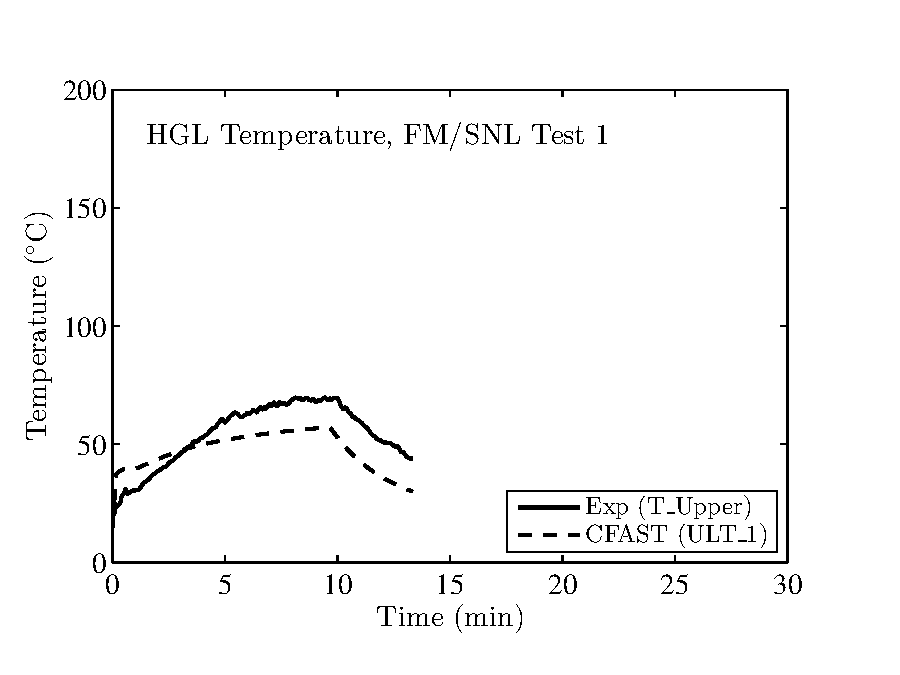
\includegraphics[width=2.6in]{FIGURES/FM_SNL/FM_SNL_01_HGL_Temp} &
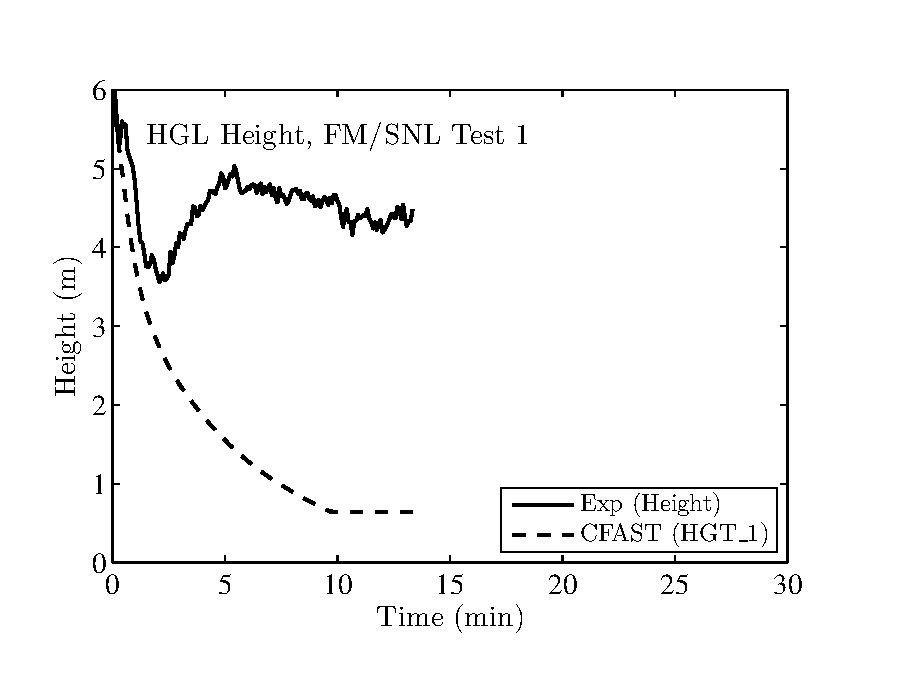
\includegraphics[width=2.6in]{FIGURES/FM_SNL/FM_SNL_01_HGL_Height} \\
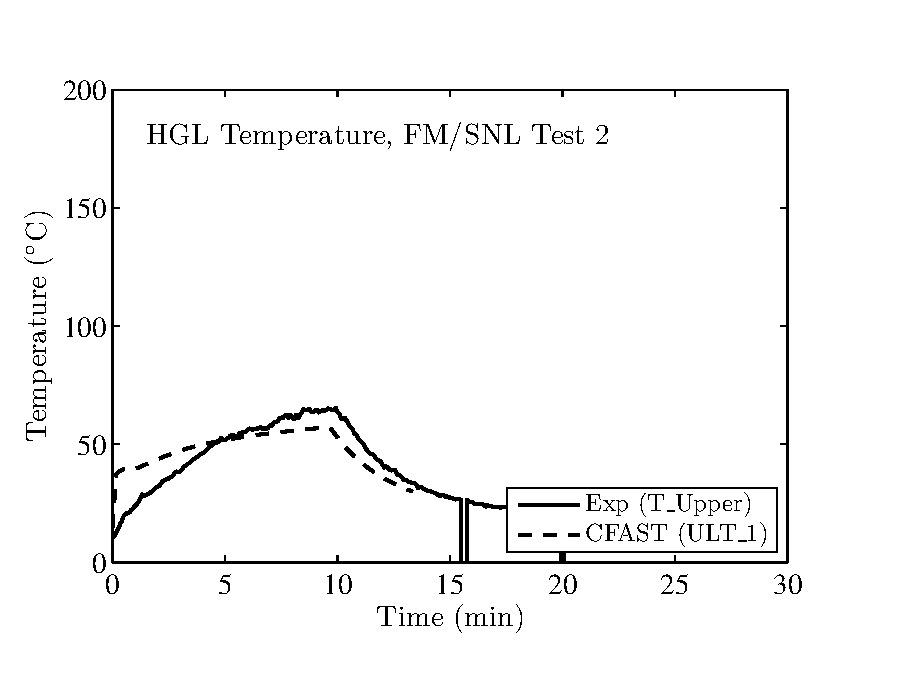
\includegraphics[width=2.6in]{FIGURES/FM_SNL/FM_SNL_02_HGL_Temp} &
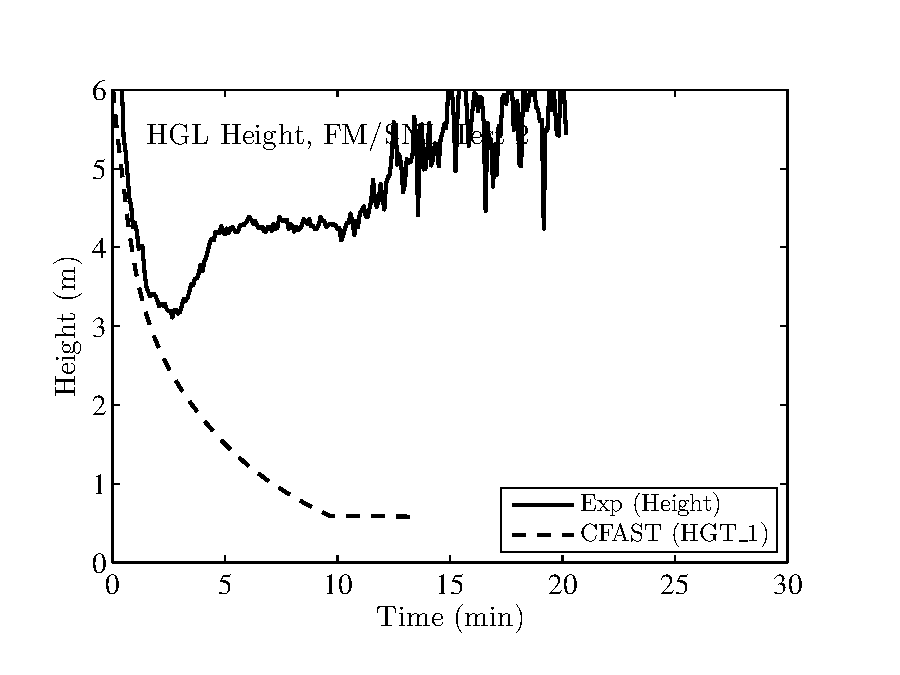
\includegraphics[width=2.6in]{FIGURES/FM_SNL/FM_SNL_02_HGL_Height} \\
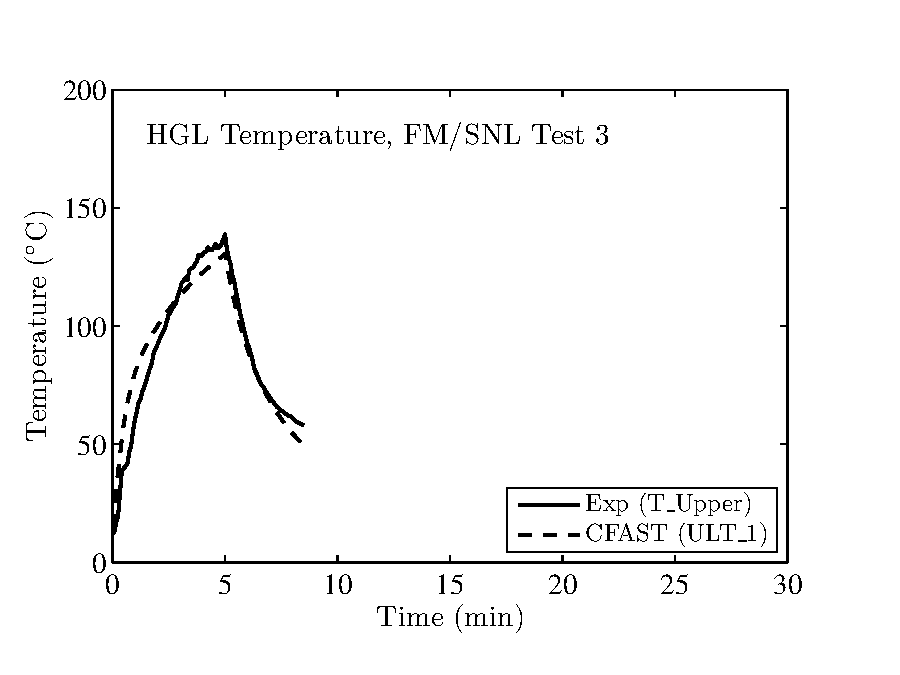
\includegraphics[width=2.6in]{FIGURES/FM_SNL/FM_SNL_03_HGL_Temp} &
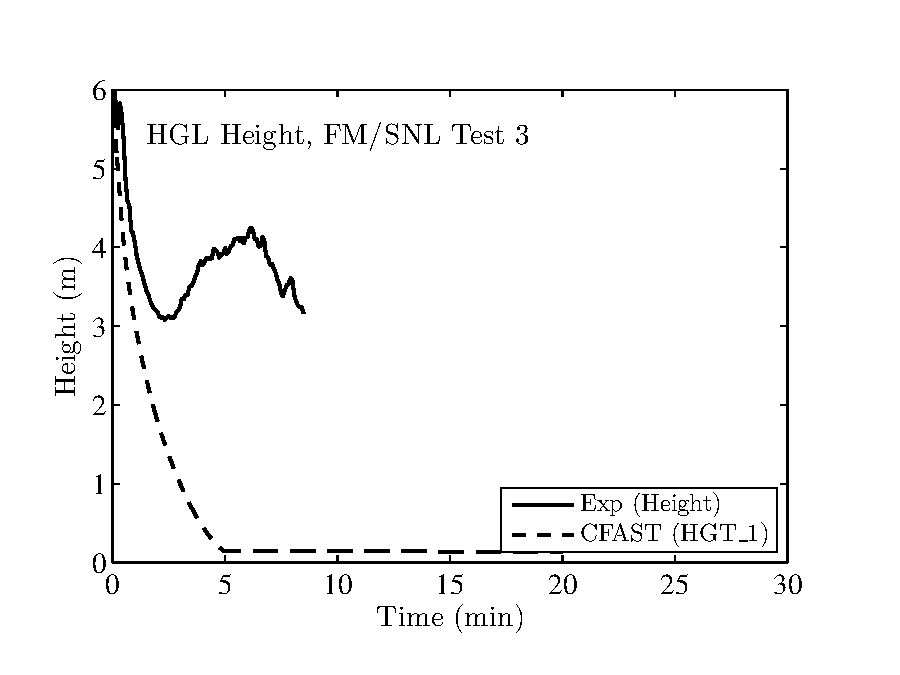
\includegraphics[width=2.6in]{FIGURES/FM_SNL/FM_SNL_03_HGL_Height} \\
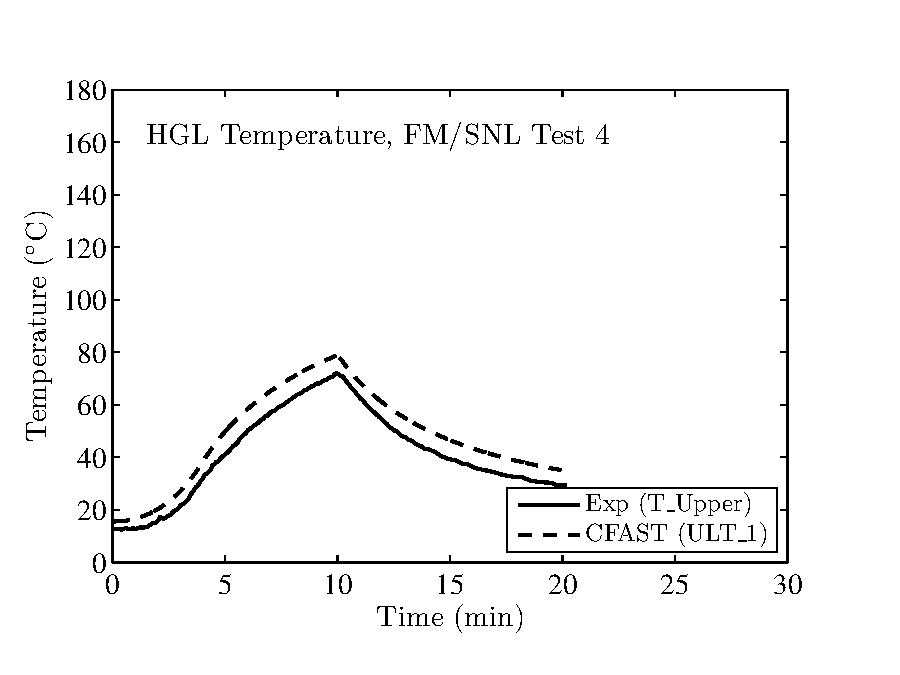
\includegraphics[width=2.6in]{FIGURES/FM_SNL/FM_SNL_04_HGL_Temp} &
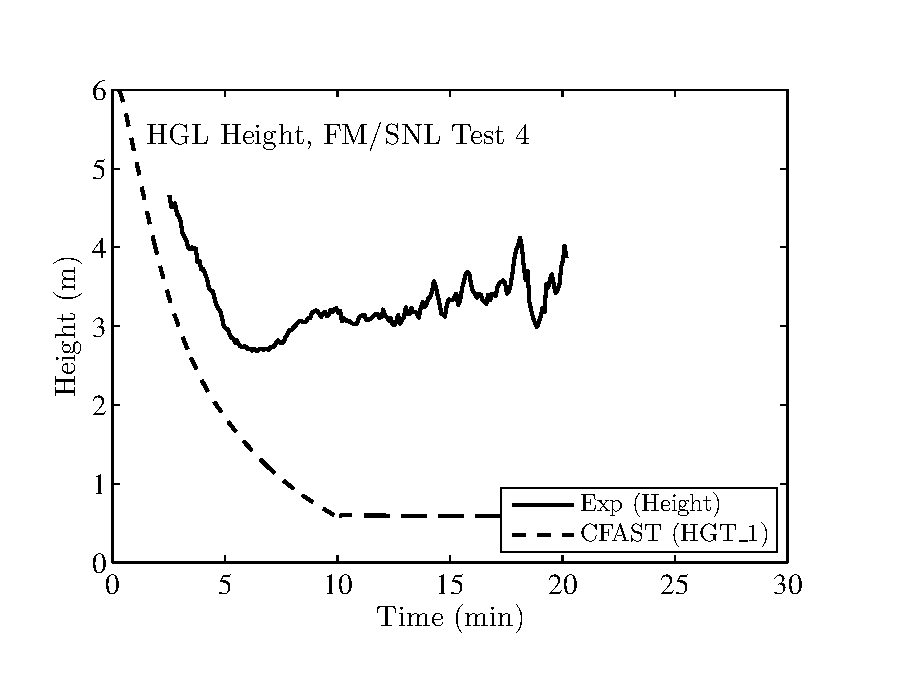
\includegraphics[width=2.6in]{FIGURES/FM_SNL/FM_SNL_04_HGL_Height} 
\end{tabular*}
\end{figure}

\begin{figure}[!ht]
\begin{tabular*}{\textwidth}{l@{\extracolsep{\fill}}r}
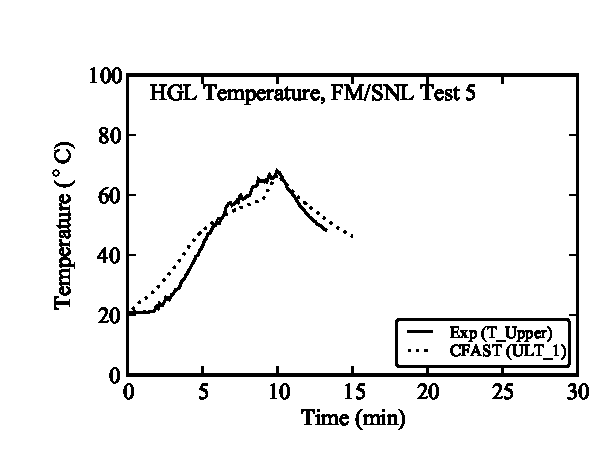
\includegraphics[width=2.6in]{FIGURES/FM_SNL/FM_SNL_05_HGL_Temp} &
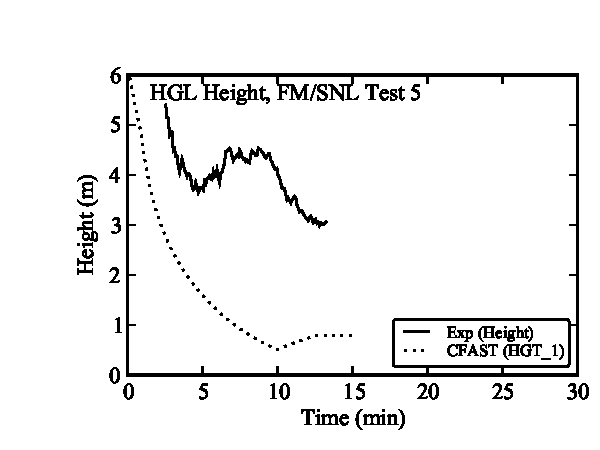
\includegraphics[width=2.6in]{FIGURES/FM_SNL/FM_SNL_05_HGL_Height} \\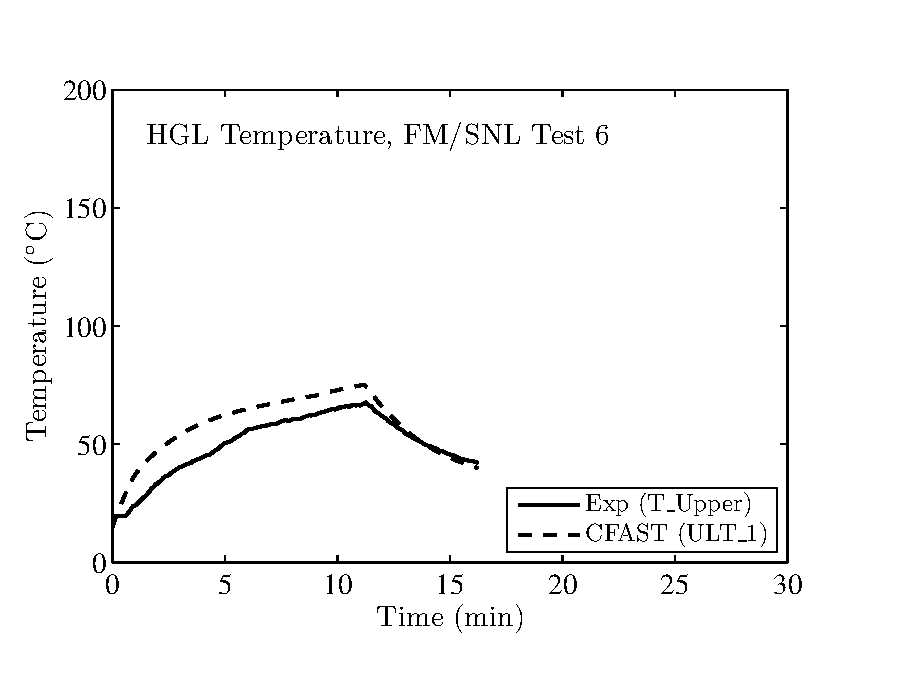
\includegraphics[width=2.6in]{FIGURES/FM_SNL/FM_SNL_06_HGL_Temp} &
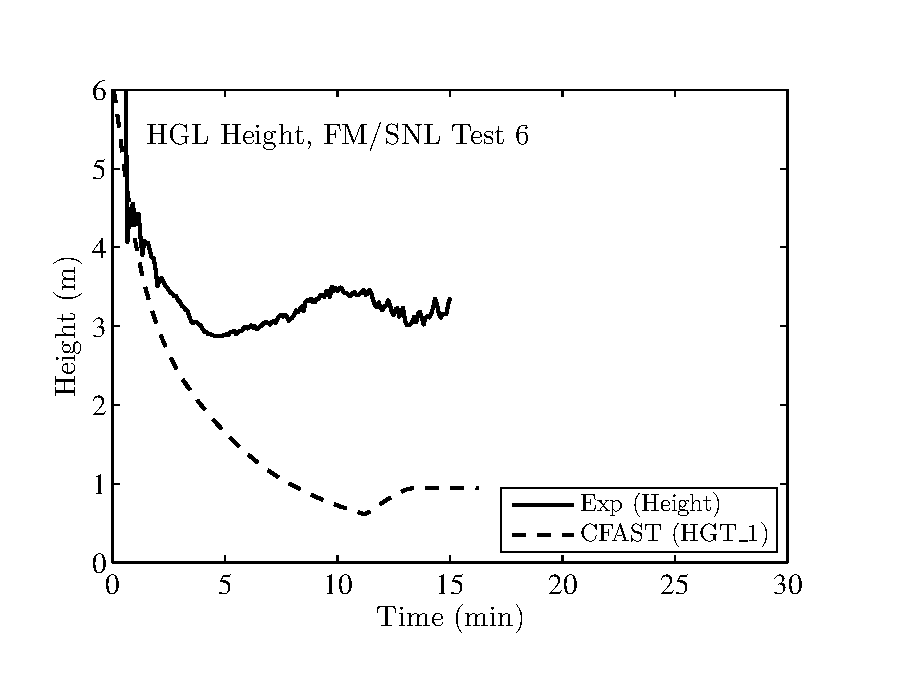
\includegraphics[width=2.6in]{FIGURES/FM_SNL/FM_SNL_06_HGL_Height} \\
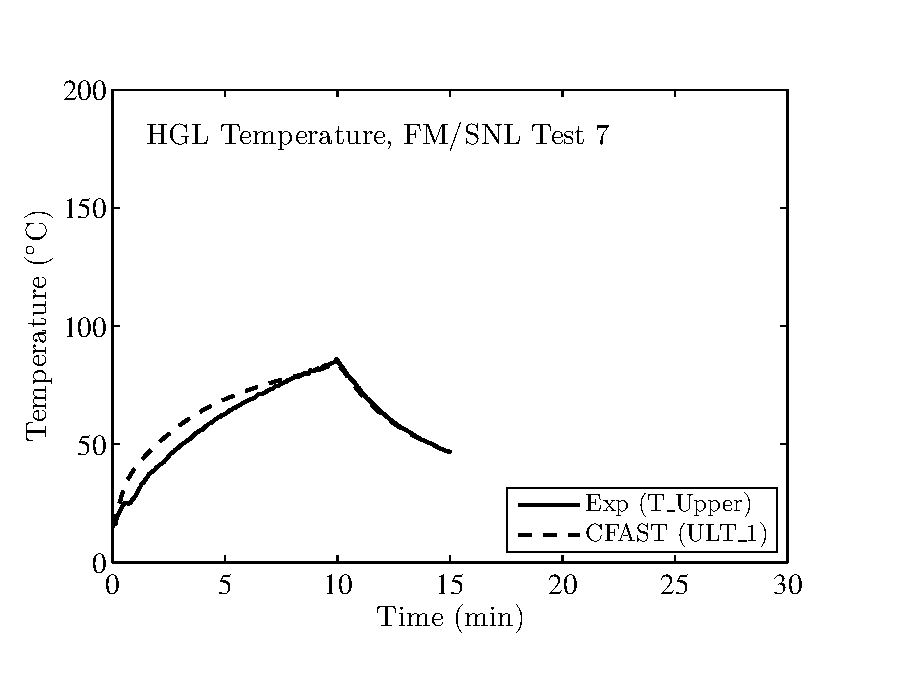
\includegraphics[width=2.6in]{FIGURES/FM_SNL/FM_SNL_07_HGL_Temp} &
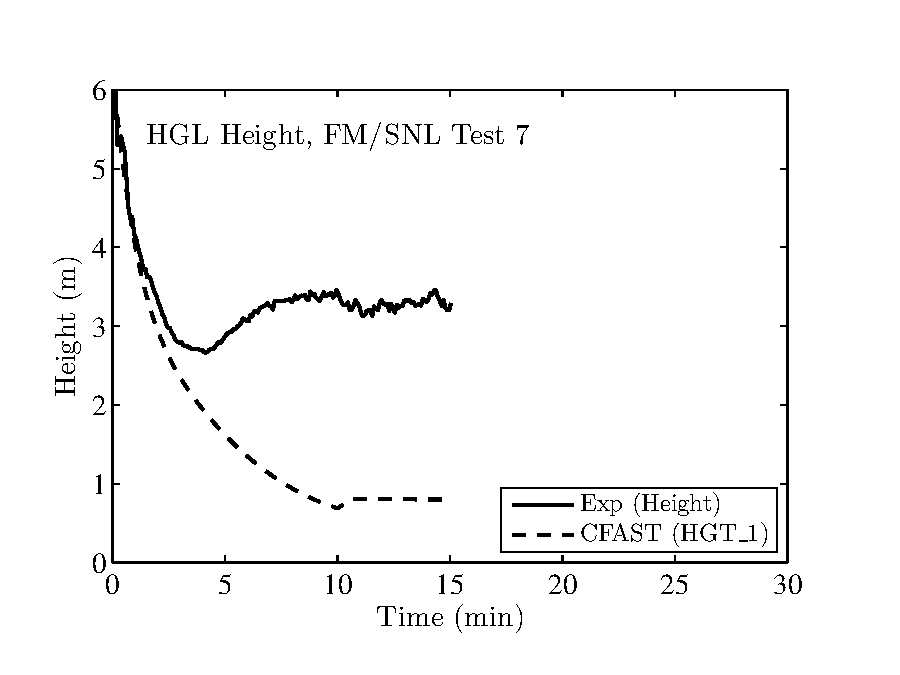
\includegraphics[width=2.6in]{FIGURES/FM_SNL/FM_SNL_07_HGL_Height} \\
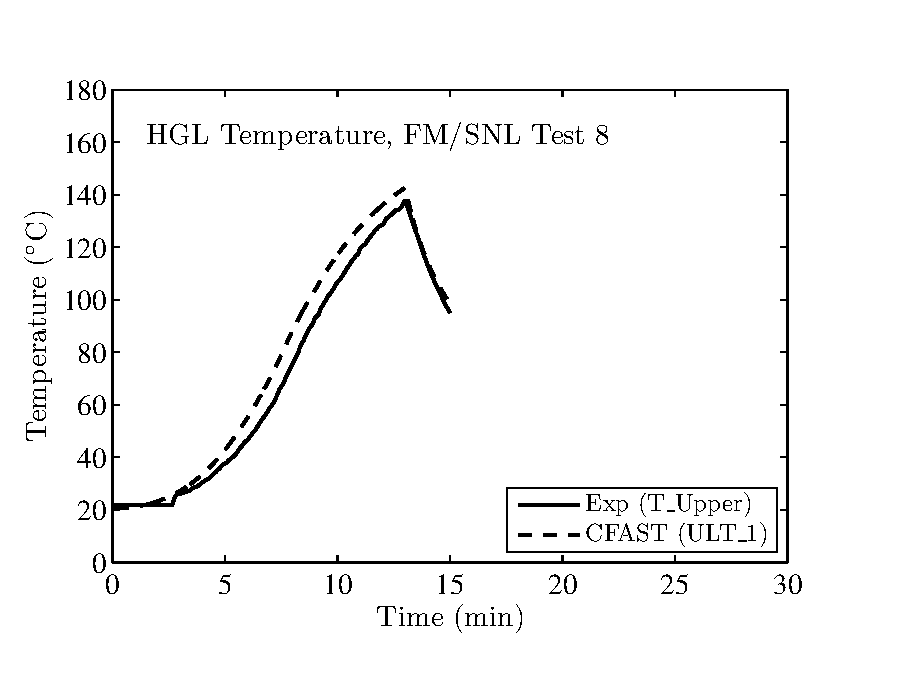
\includegraphics[width=2.6in]{FIGURES/FM_SNL/FM_SNL_08_HGL_Temp} &
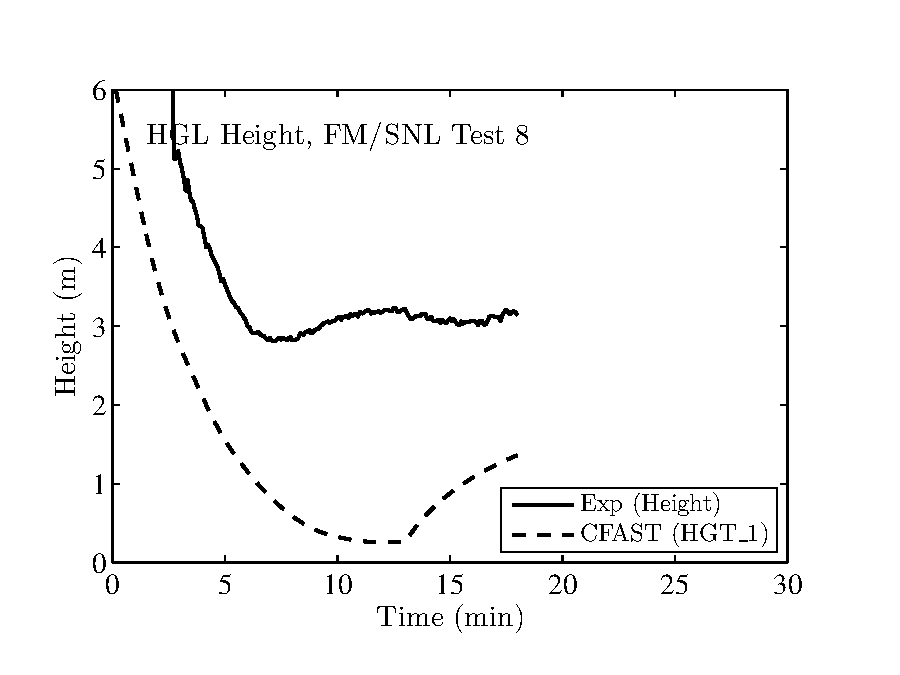
\includegraphics[width=2.6in]{FIGURES/FM_SNL/FM_SNL_08_HGL_Height}
\end{tabular*}
\end{figure}

\begin{figure}[!ht]
\begin{tabular*}{\textwidth}{l@{\extracolsep{\fill}}r}
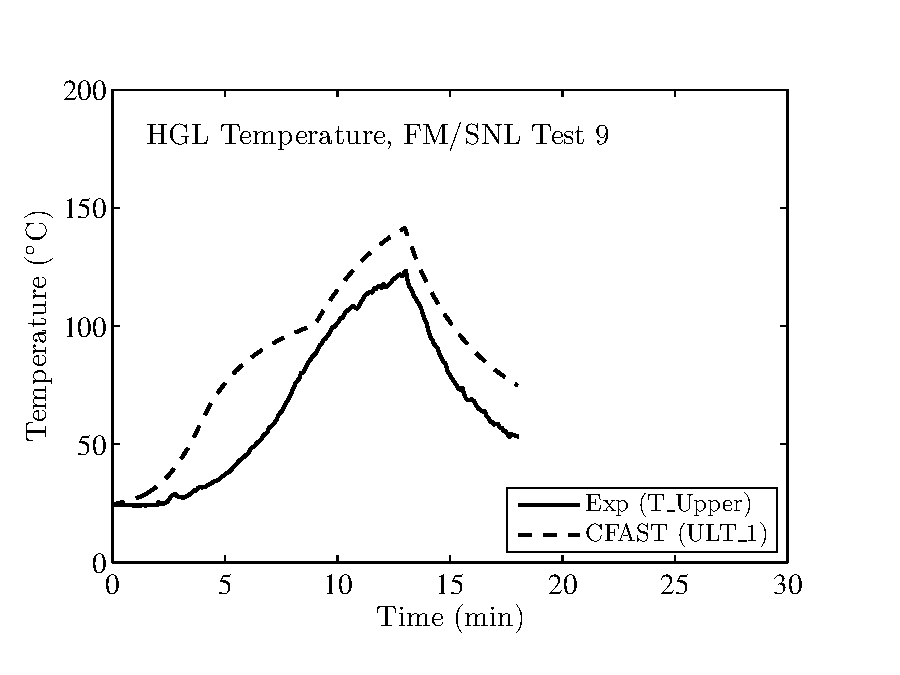
\includegraphics[width=2.6in]{FIGURES/FM_SNL/FM_SNL_09_HGL_Temp} &
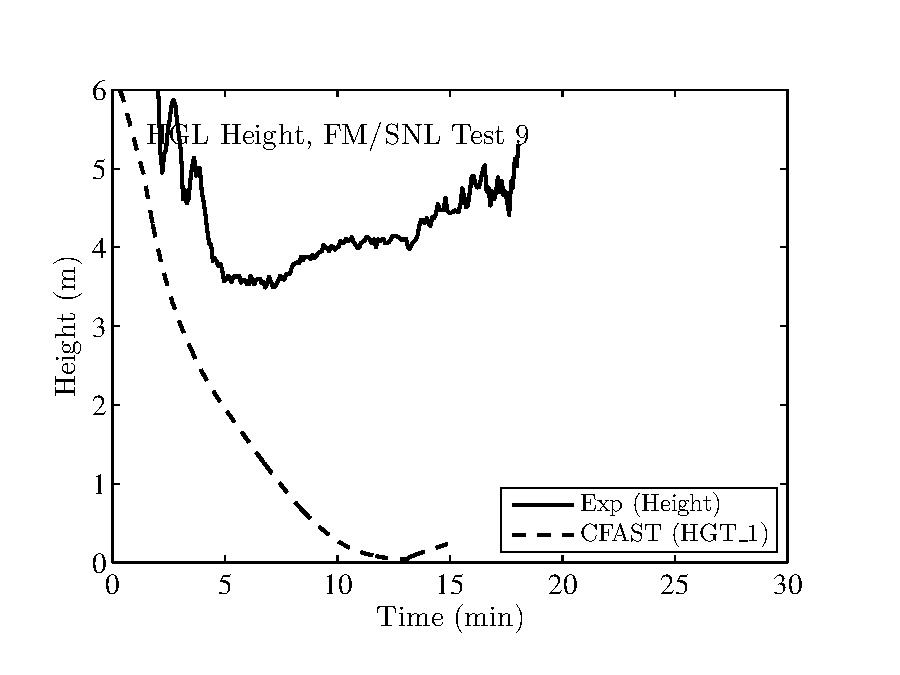
\includegraphics[width=2.6in]{FIGURES/FM_SNL/FM_SNL_09_HGL_Height} \\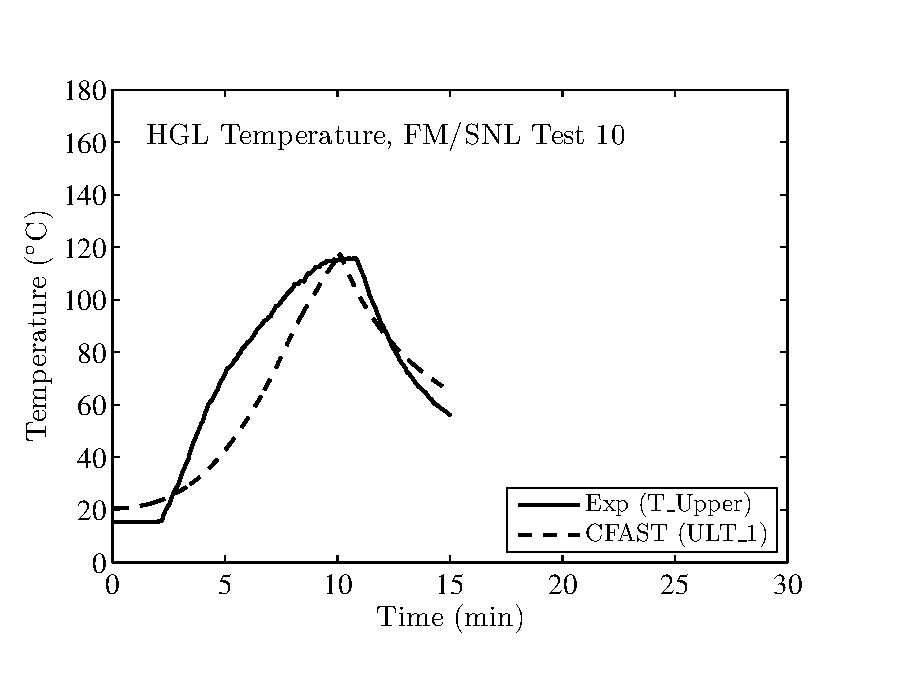
\includegraphics[width=2.6in]{FIGURES/FM_SNL/FM_SNL_10_HGL_Temp} &
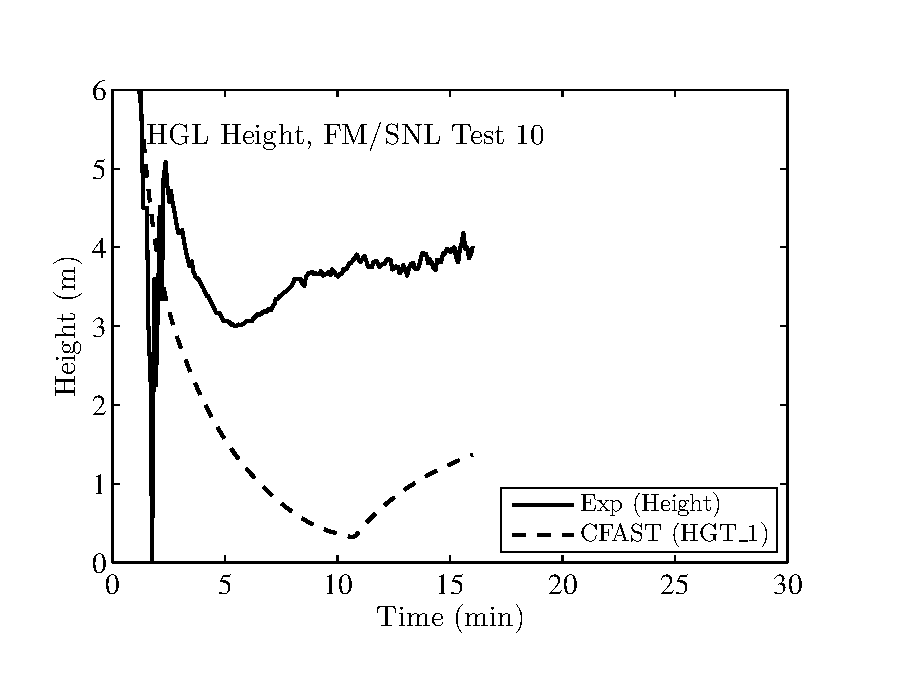
\includegraphics[width=2.6in]{FIGURES/FM_SNL/FM_SNL_10_HGL_Height} \\
\includegraphics[width=2.6in]{FIGURES/FM_SNL/FM_SNL_11_HGL_Temp} &
\includegraphics[width=2.6in]{FIGURES/FM_SNL/FM_SNL_11_HGL_Height} \\
\includegraphics[width=2.6in]{FIGURES/FM_SNL/FM_SNL_12_HGL_Temp} &
\includegraphics[width=2.6in]{FIGURES/FM_SNL/FM_SNL_12_HGL_Height}
\end{tabular*}
\end{figure}

\begin{figure}[!ht]
\begin{tabular*}{\textwidth}{l@{\extracolsep{\fill}}r}
\includegraphics[width=2.6in]{FIGURES/FM_SNL/FM_SNL_13_HGL_Temp} &
\includegraphics[width=2.6in]{FIGURES/FM_SNL/FM_SNL_13_HGL_Height} \\
\includegraphics[width=2.6in]{FIGURES/FM_SNL/FM_SNL_14_HGL_Temp} &
\includegraphics[width=2.6in]{FIGURES/FM_SNL/FM_SNL_14_HGL_Height} \\
\includegraphics[width=2.6in]{FIGURES/FM_SNL/FM_SNL_15_HGL_Temp} &
\includegraphics[width=2.6in]{FIGURES/FM_SNL/FM_SNL_15_HGL_Height} \\
\includegraphics[width=2.6in]{FIGURES/FM_SNL/FM_SNL_16_HGL_Temp} &
\includegraphics[width=2.6in]{FIGURES/FM_SNL/FM_SNL_16_HGL_Height} 
\end{tabular*}\end{figure}

\begin{figure}[!ht]
\begin{tabular*}{\textwidth}{l@{\extracolsep{\fill}}r}
\includegraphics[width=2.6in]{FIGURES/FM_SNL/FM_SNL_17_HGL_Temp} &
\includegraphics[width=2.6in]{FIGURES/FM_SNL/FM_SNL_17_HGL_Height} \\
\includegraphics[width=2.6in]{FIGURES/FM_SNL/FM_SNL_21_HGL_Temp} &
\includegraphics[width=2.6in]{FIGURES/FM_SNL/FM_SNL_21_HGL_Height} \\
\includegraphics[width=2.6in]{FIGURES/FM_SNL/FM_SNL_22_HGL_Temp} &
\includegraphics[width=2.6in]{FIGURES/FM_SNL/FM_SNL_22_HGL_Height}
\end{tabular*}
\end{figure}

\begin{figure}[!ht]
\begin{tabular*}{\textwidth}{l@{\extracolsep{\fill}}r}
\includegraphics[width=2.6in]{FIGURES/FM_SNL/FM_SNL_01_Plume_Temperature} &
\includegraphics[width=2.6in]{FIGURES/FM_SNL/FM_SNL_02_Plume_Temperature} \\
\includegraphics[width=2.6in]{FIGURES/FM_SNL/FM_SNL_03_Plume_Temperature} &
\includegraphics[width=2.6in]{FIGURES/FM_SNL/FM_SNL_04_Plume_Temperature} \\
\includegraphics[width=2.6in]{FIGURES/FM_SNL/FM_SNL_05_Plume_Temperature} &
\includegraphics[width=2.6in]{FIGURES/FM_SNL/FM_SNL_06_Plume_Temperature} \\
\includegraphics[width=2.6in]{FIGURES/FM_SNL/FM_SNL_07_Plume_Temperature} &
\includegraphics[width=2.6in]{FIGURES/FM_SNL/FM_SNL_08_Plume_Temperature} 
\end{tabular*}
\end{figure}

\begin{figure}[!ht]
\begin{tabular*}{\textwidth}{l@{\extracolsep{\fill}}r}
\includegraphics[width=2.6in]{FIGURES/FM_SNL/FM_SNL_09_Plume_Temperature} &
\includegraphics[width=2.6in]{FIGURES/FM_SNL/FM_SNL_10_Plume_Temperature} \\
\includegraphics[width=2.6in]{FIGURES/FM_SNL/FM_SNL_11_Plume_Temperature} &
\includegraphics[width=2.6in]{FIGURES/FM_SNL/FM_SNL_12_Plume_Temperature} \\
\includegraphics[width=2.6in]{FIGURES/FM_SNL/FM_SNL_13_Plume_Temperature} &
\includegraphics[width=2.6in]{FIGURES/FM_SNL/FM_SNL_14_Plume_Temperature} \\
\includegraphics[width=2.6in]{FIGURES/FM_SNL/FM_SNL_15_Plume_Temperature} &
\includegraphics[width=2.6in]{FIGURES/FM_SNL/FM_SNL_16_Plume_Temperature} 
\end{tabular*}
\end{figure}

\begin{figure}[!ht]
\begin{center}
\includegraphics[width=2.6in]{FIGURES/FM_SNL/FM_SNL_17_Plume_Temperature} \\
\includegraphics[width=2.6in]{FIGURES/FM_SNL/FM_SNL_21_Plume_Temperature} \\
\includegraphics[width=2.6in]{FIGURES/FM_SNL/FM_SNL_22_Plume_Temperature} 
\end{center}
\end{figure}

\begin{figure}[!ht]
\begin{tabular*}{\textwidth}{l@{\extracolsep{\fill}}r}
\includegraphics[width=2.6in]{FIGURES/FM_SNL/FM_SNL_01_Ceiling_Jet} &
\includegraphics[width=2.6in]{FIGURES/FM_SNL/FM_SNL_02_Ceiling_Jet} \\
\includegraphics[width=2.6in]{FIGURES/FM_SNL/FM_SNL_03_Ceiling_Jet} &
\includegraphics[width=2.6in]{FIGURES/FM_SNL/FM_SNL_04_Ceiling_Jet} \\
\includegraphics[width=2.6in]{FIGURES/FM_SNL/FM_SNL_05_Ceiling_Jet} &
\includegraphics[width=2.6in]{FIGURES/FM_SNL/FM_SNL_06_Ceiling_Jet} \\
\includegraphics[width=2.6in]{FIGURES/FM_SNL/FM_SNL_07_Ceiling_Jet} &
\includegraphics[width=2.6in]{FIGURES/FM_SNL/FM_SNL_08_Ceiling_Jet} 
\end{tabular*}
\end{figure}

\begin{figure}[!ht]
\begin{tabular*}{\textwidth}{l@{\extracolsep{\fill}}r}
\includegraphics[width=2.6in]{FIGURES/FM_SNL/FM_SNL_09_Ceiling_Jet} &
\includegraphics[width=2.6in]{FIGURES/FM_SNL/FM_SNL_10_Ceiling_Jet} \\
\includegraphics[width=2.6in]{FIGURES/FM_SNL/FM_SNL_11_Ceiling_Jet} &
\includegraphics[width=2.6in]{FIGURES/FM_SNL/FM_SNL_12_Ceiling_Jet} \\
\includegraphics[width=2.6in]{FIGURES/FM_SNL/FM_SNL_13_Ceiling_Jet} &
\includegraphics[width=2.6in]{FIGURES/FM_SNL/FM_SNL_14_Ceiling_Jet} \\
\includegraphics[width=2.6in]{FIGURES/FM_SNL/FM_SNL_15_Ceiling_Jet} &
\includegraphics[width=2.6in]{FIGURES/FM_SNL/FM_SNL_16_Ceiling_Jet} 
\end{tabular*}
\end{figure}

\begin{figure}[!ht]
\begin{center}
\includegraphics[width=2.6in]{FIGURES/FM_SNL/FM_SNL_17_Ceiling_Jet} \\
\includegraphics[width=2.6in]{FIGURES/FM_SNL/FM_SNL_21_Ceiling_Jet} \\
\includegraphics[width=2.6in]{FIGURES/FM_SNL/FM_SNL_22_Ceiling_Jet} 
\end{center}
\end{figure}

\clearpage

\subsection{iBMB Compartment Tests}

\begin{figure}[!ht]
\begin{tabular*}{\textwidth}{l@{\extracolsep{\fill}}r}
\includegraphics[width=2.6in]{FIGURES/iBMB/iBMB_Pool_HGL_Temp} &
\includegraphics[width=2.6in]{FIGURES/iBMB/iBMB_Pool_HGL_Height} \\
\includegraphics[width=2.6in]{FIGURES/iBMB/iBMB_Cable_HGL_Temp} &
\includegraphics[width=2.6in]{FIGURES/iBMB/iBMB_Cable_HGL_Height} 
\end{tabular*}
\end{figure}

\clearpage

\subsection{LLNL Enclosure Series}

\begin{figure}[!ht]
\begin{tabular*}{\textwidth}{l@{\extracolsep{\fill}}r}
\includegraphics[width=2.6in]{FIGURES/LLNL_Enclosure/LLNL_01_Temp} &
\includegraphics[width=2.6in]{FIGURES/LLNL_Enclosure/LLNL_02_Temp} \\
\includegraphics[width=2.6in]{FIGURES/LLNL_Enclosure/LLNL_03_Temp} &
\includegraphics[width=2.6in]{FIGURES/LLNL_Enclosure/LLNL_04_Temp} \\
\includegraphics[width=2.6in]{FIGURES/LLNL_Enclosure/LLNL_05_Temp} &
\includegraphics[width=2.6in]{FIGURES/LLNL_Enclosure/LLNL_06_Temp} \\
\includegraphics[width=2.6in]{FIGURES/LLNL_Enclosure/LLNL_07_Temp} &
\includegraphics[width=2.6in]{FIGURES/LLNL_Enclosure/LLNL_08_Temp}
\end{tabular*}
\label{LLNL_Enclosure_Temp_1}
\end{figure}

\begin{figure}[!ht]
\begin{tabular*}{\textwidth}{l@{\extracolsep{\fill}}r}
\includegraphics[width=2.6in]{FIGURES/LLNL_Enclosure/LLNL_09_Temp} &
\includegraphics[width=2.6in]{FIGURES/LLNL_Enclosure/LLNL_10_Temp} \\
\includegraphics[width=2.6in]{FIGURES/LLNL_Enclosure/LLNL_11_Temp} &
\includegraphics[width=2.6in]{FIGURES/LLNL_Enclosure/LLNL_12_Temp} \\
\includegraphics[width=2.6in]{FIGURES/LLNL_Enclosure/LLNL_13_Temp} &
\includegraphics[width=2.6in]{FIGURES/LLNL_Enclosure/LLNL_14_Temp} \\
 \includegraphics[width=2.6in]{FIGURES/LLNL_Enclosure/LLNL_15_Temp} &
\includegraphics[width=2.6in]{FIGURES/LLNL_Enclosure/LLNL_16_Temp}
\end{tabular*}
\label{LLNL_Enclosure_Temp_2}
\end{figure}

\begin{figure}[!ht]
\begin{tabular*}{\textwidth}{l@{\extracolsep{\fill}}r}
 \includegraphics[width=2.6in]{FIGURES/LLNL_Enclosure/LLNL_17_Temp} &
 \includegraphics[width=2.6in]{FIGURES/LLNL_Enclosure/LLNL_18_Temp} \\
\includegraphics[width=2.6in]{FIGURES/LLNL_Enclosure/LLNL_19_Temp} &
 \includegraphics[width=2.6in]{FIGURES/LLNL_Enclosure/LLNL_20_Temp} \\
\includegraphics[width=2.6in]{FIGURES/LLNL_Enclosure/LLNL_21_Temp} &
\includegraphics[width=2.6in]{FIGURES/LLNL_Enclosure/LLNL_22_Temp} \\
\includegraphics[width=2.6in]{FIGURES/LLNL_Enclosure/LLNL_23_Temp} &
\includegraphics[width=2.6in]{FIGURES/LLNL_Enclosure/LLNL_24_Temp}
\end{tabular*}
\label{LLNL_Enclosure_Temp_3}
\end{figure}

\begin{figure}[!ht]
\begin{tabular*}{\textwidth}{l@{\extracolsep{\fill}}r}
\includegraphics[width=2.6in]{FIGURES/LLNL_Enclosure/LLNL_25_Temp} &
\includegraphics[width=2.6in]{FIGURES/LLNL_Enclosure/LLNL_26_Temp} \\
\includegraphics[width=2.6in]{FIGURES/LLNL_Enclosure/LLNL_27_Temp} &
\includegraphics[width=2.6in]{FIGURES/LLNL_Enclosure/LLNL_28_Temp} \\
\includegraphics[width=2.6in]{FIGURES/LLNL_Enclosure/LLNL_29_Temp} &
\includegraphics[width=2.6in]{FIGURES/LLNL_Enclosure/LLNL_30_Temp} \\
\includegraphics[width=2.6in]{FIGURES/LLNL_Enclosure/LLNL_31_Temp} &
\includegraphics[width=2.6in]{FIGURES/LLNL_Enclosure/LLNL_32_Temp}
\end{tabular*}
\label{LLNL_Enclosure_Temp_4}
\end{figure}

\begin{figure}[!ht]
\begin{tabular*}{\textwidth}{l@{\extracolsep{\fill}}r}
\includegraphics[width=2.6in]{FIGURES/LLNL_Enclosure/LLNL_33_Temp} &
\includegraphics[width=2.6in]{FIGURES/LLNL_Enclosure/LLNL_34_Temp} \\
\includegraphics[width=2.6in]{FIGURES/LLNL_Enclosure/LLNL_35_Temp} &
\includegraphics[width=2.6in]{FIGURES/LLNL_Enclosure/LLNL_36_Temp} \\
\includegraphics[width=2.6in]{FIGURES/LLNL_Enclosure/LLNL_37_Temp} &
\includegraphics[width=2.6in]{FIGURES/LLNL_Enclosure/LLNL_38_Temp} \\
\includegraphics[width=2.6in]{FIGURES/LLNL_Enclosure/LLNL_39_Temp} &
\includegraphics[width=2.6in]{FIGURES/LLNL_Enclosure/LLNL_40_Temp}
\end{tabular*}
\label{LLNL_Enclosure_Temp_5}
\end{figure}

\begin{figure}[!ht]
\begin{tabular*}{\textwidth}{l@{\extracolsep{\fill}}r}
\includegraphics[width=2.6in]{FIGURES/LLNL_Enclosure/LLNL_41_Temp} &
\includegraphics[width=2.6in]{FIGURES/LLNL_Enclosure/LLNL_42_Temp} \\
\includegraphics[width=2.6in]{FIGURES/LLNL_Enclosure/LLNL_43_Temp} &
\includegraphics[width=2.6in]{FIGURES/LLNL_Enclosure/LLNL_44_Temp} \\
\includegraphics[width=2.6in]{FIGURES/LLNL_Enclosure/LLNL_45_Temp} &
\includegraphics[width=2.6in]{FIGURES/LLNL_Enclosure/LLNL_46_Temp} \\
\includegraphics[width=2.6in]{FIGURES/LLNL_Enclosure/LLNL_47_Temp} &
\includegraphics[width=2.6in]{FIGURES/LLNL_Enclosure/LLNL_48_Temp}
\end{tabular*}
\label{LLNL_Enclosure_Temp_6}
\end{figure}

\begin{figure}[!ht]
\begin{tabular*}{\textwidth}{l@{\extracolsep{\fill}}r}
\includegraphics[width=2.6in]{FIGURES/LLNL_Enclosure/LLNL_49_Temp} &
\includegraphics[width=2.6in]{FIGURES/LLNL_Enclosure/LLNL_50_Temp} \\
\includegraphics[width=2.6in]{FIGURES/LLNL_Enclosure/LLNL_51_Temp} &
\includegraphics[width=2.6in]{FIGURES/LLNL_Enclosure/LLNL_52_Temp} \\
\includegraphics[width=2.6in]{FIGURES/LLNL_Enclosure/LLNL_53_Temp} &
\includegraphics[width=2.6in]{FIGURES/LLNL_Enclosure/LLNL_54_Temp} \\
\includegraphics[width=2.6in]{FIGURES/LLNL_Enclosure/LLNL_55_Temp} &
\includegraphics[width=2.6in]{FIGURES/LLNL_Enclosure/LLNL_56_Temp}
\end{tabular*}
\label{LLNL_Enclosure_Temp_7}
\end{figure}

\begin{figure}[!ht]
\begin{tabular*}{\textwidth}{l@{\extracolsep{\fill}}r}
\includegraphics[width=2.6in]{FIGURES/LLNL_Enclosure/LLNL_57_Temp} &
\includegraphics[width=2.6in]{FIGURES/LLNL_Enclosure/LLNL_58_Temp} \\
\includegraphics[width=2.6in]{FIGURES/LLNL_Enclosure/LLNL_59_Temp} &
\includegraphics[width=2.6in]{FIGURES/LLNL_Enclosure/LLNL_60_Temp} \\
\includegraphics[width=2.6in]{FIGURES/LLNL_Enclosure/LLNL_61_Temp} &
\includegraphics[width=2.6in]{FIGURES/LLNL_Enclosure/LLNL_62_Temp} \\
\includegraphics[width=2.6in]{FIGURES/LLNL_Enclosure/LLNL_63_Temp} &
\includegraphics[width=2.6in]{FIGURES/LLNL_Enclosure/LLNL_64_Temp}
\end{tabular*}
\label{LLNL_Enclosure_Temp_8}
\end{figure}

\clearpage

\subsection{NBS Multi-Compartment Test Series}

\begin{figure}[!ht]
\begin{tabular*}{\textwidth}{l@{\extracolsep{\fill}}r}
\includegraphics[width=2.6in]{FIGURES/NBS/NBS_100A_Tree_1_HGL_Temp} &
\includegraphics[width=2.6in]{FIGURES/NBS/NBS_100A_Tree_1_HGL_Height} \\
\includegraphics[width=2.6in]{FIGURES/NBS/NBS_100A_Tree_4_HGL_Temp} &
\includegraphics[width=2.6in]{FIGURES/NBS/NBS_100A_Tree_4_HGL_Height} \\
\includegraphics[width=2.6in]{FIGURES/NBS/NBS_100A_Tree_5_HGL_Temp} &
\includegraphics[width=2.6in]{FIGURES/NBS/NBS_100A_Tree_5_HGL_Height}\\
\includegraphics[width=2.6in]{FIGURES/NBS/NBS_100A_Tree_6_HGL_Temp} &
\includegraphics[width=2.6in]{FIGURES/NBS/NBS_100A_Tree_6_HGL_Height}
\end{tabular*}
\end{figure}

\begin{figure}[!ht]
\begin{tabular*}{\textwidth}{l@{\extracolsep{\fill}}r}
\includegraphics[width=2.6in]{FIGURES/NBS/NBS_100O_Tree_1_HGL_Temp} &
\includegraphics[width=2.6in]{FIGURES/NBS/NBS_100O_Tree_1_HGL_Height} \\
\includegraphics[width=2.6in]{FIGURES/NBS/NBS_100O_Tree_4_HGL_Temp} &
\includegraphics[width=2.6in]{FIGURES/NBS/NBS_100O_Tree_4_HGL_Height} \\
\includegraphics[width=2.6in]{FIGURES/NBS/NBS_100O_Tree_5_HGL_Temp} &
\includegraphics[width=2.6in]{FIGURES/NBS/NBS_100O_Tree_5_HGL_Height}\\
\includegraphics[width=2.6in]{FIGURES/NBS/NBS_100O_Tree_6_HGL_Temp} &
\includegraphics[width=2.6in]{FIGURES/NBS/NBS_100O_Tree_6_HGL_Height}
\end{tabular*}
\end{figure}

\begin{figure}[!ht]
\begin{tabular*}{\textwidth}{l@{\extracolsep{\fill}}r}
\includegraphics[width=2.6in]{FIGURES/NBS/NBS_100Z_Tree_1_HGL_Temp} &
\includegraphics[width=2.6in]{FIGURES/NBS/NBS_100Z_Tree_1_HGL_Height} \\
\includegraphics[width=2.6in]{FIGURES/NBS/NBS_100Z_Tree_4_HGL_Temp} &
\includegraphics[width=2.6in]{FIGURES/NBS/NBS_100Z_Tree_4_HGL_Height} \\
\includegraphics[width=2.6in]{FIGURES/NBS/NBS_100Z_Tree_5_HGL_Temp} &
\includegraphics[width=2.6in]{FIGURES/NBS/NBS_100Z_Tree_5_HGL_Height}\\
\includegraphics[width=2.6in]{FIGURES/NBS/NBS_100Z_Tree_7_HGL_Temp} &
\includegraphics[width=2.6in]{FIGURES/NBS/NBS_100Z_Tree_7_HGL_Height}
\end{tabular*}
\end{figure}

\clearpage

\subsection{NIST Smoke Alarm Experiments}

\begin{figure}[h!]
\begin{tabular*}{\textwidth}{l@{\extracolsep{\fill}}r}
\includegraphics[width=2.6in]{FIGURES/NIST_Dunes_2000/NIST_Dunes_2000_SDC02_Ceiling_Jet} &
\includegraphics[width=2.6in]{FIGURES/NIST_Dunes_2000/NIST_Dunes_2000_SDC05_Ceiling_Jet} \\
\includegraphics[width=2.6in]{FIGURES/NIST_Dunes_2000/NIST_Dunes_2000_SDC07_Ceiling_Jet} &
\includegraphics[width=2.6in]{FIGURES/NIST_Dunes_2000/NIST_Dunes_2000_SDC10_Ceiling_Jet} \\
\includegraphics[width=2.6in]{FIGURES/NIST_Dunes_2000/NIST_Dunes_2000_SDC33_Ceiling_Jet} &
\includegraphics[width=2.6in]{FIGURES/NIST_Dunes_2000/NIST_Dunes_2000_SDC35_Ceiling_Jet} \\
\includegraphics[width=2.6in]{FIGURES/NIST_Dunes_2000/NIST_Dunes_2000_SDC39_Ceiling_Jet}
\end{tabular*}
\label{NIST_Dunes_2000_Ceiling_Jet}
\end{figure}

\clearpage

\subsection{NIST/NRC Test Series}

\begin{figure}[!ht]
\begin{tabular*}{\textwidth}{l@{\extracolsep{\fill}}r}
\includegraphics[width=2.6in]{FIGURES/NIST_NRC/NIST_NRC_01_HGL_Temp} &
\includegraphics[width=2.6in]{FIGURES/NIST_NRC/NIST_NRC_01_HGL_Height} \\
\includegraphics[width=2.6in]{FIGURES/NIST_NRC/NIST_NRC_07_HGL_Temp} &
\includegraphics[width=2.6in]{FIGURES/NIST_NRC/NIST_NRC_07_HGL_Height} \\
\includegraphics[width=2.6in]{FIGURES/NIST_NRC/NIST_NRC_02_HGL_Temp} &
\includegraphics[width=2.6in]{FIGURES/NIST_NRC/NIST_NRC_02_HGL_Height} \\
\includegraphics[width=2.6in]{FIGURES/NIST_NRC/NIST_NRC_08_HGL_Temp} &
\includegraphics[width=2.6in]{FIGURES/NIST_NRC/NIST_NRC_08_HGL_Height}
\end{tabular*}
\end{figure}

\begin{figure}[!ht]
\begin{tabular*}{\textwidth}{l@{\extracolsep{\fill}}r}
\includegraphics[width=2.6in]{FIGURES/NIST_NRC/NIST_NRC_04_HGL_Temp} &
\includegraphics[width=2.6in]{FIGURES/NIST_NRC/NIST_NRC_04_HGL_Height} \\
\includegraphics[width=2.6in]{FIGURES/NIST_NRC/NIST_NRC_10_HGL_Temp} &
\includegraphics[width=2.6in]{FIGURES/NIST_NRC/NIST_NRC_10_HGL_Height} \\
\includegraphics[width=2.6in]{FIGURES/NIST_NRC/NIST_NRC_13_HGL_Temp} &
\includegraphics[width=2.6in]{FIGURES/NIST_NRC/NIST_NRC_13_HGL_Height} \\
\includegraphics[width=2.6in]{FIGURES/NIST_NRC/NIST_NRC_16_HGL_Temp} &
\includegraphics[width=2.6in]{FIGURES/NIST_NRC/NIST_NRC_16_HGL_Height}
\end{tabular*}
\end{figure}

\clearpage

\begin{figure}[!ht]
\begin{tabular*}{\textwidth}{l@{\extracolsep{\fill}}r}
\includegraphics[width=2.6in]{FIGURES/NIST_NRC/NIST_NRC_17_HGL_Temp} &
\includegraphics[width=2.6in]{FIGURES/NIST_NRC/NIST_NRC_17_HGL_Height} \\
\multicolumn{2}{c}{Open Door Tests to follow} \\
\includegraphics[width=2.6in]{FIGURES/NIST_NRC/NIST_NRC_03_HGL_Temp} &
\includegraphics[width=2.6in]{FIGURES/NIST_NRC/NIST_NRC_03_HGL_Height} \\
\includegraphics[width=2.6in]{FIGURES/NIST_NRC/NIST_NRC_09_HGL_Temp} &
\includegraphics[width=2.6in]{FIGURES/NIST_NRC/NIST_NRC_09_HGL_Height}
\end{tabular*}
\end{figure}

\begin{figure}[!ht]
\begin{tabular*}{\textwidth}{l@{\extracolsep{\fill}}r}
\includegraphics[width=2.6in]{FIGURES/NIST_NRC/NIST_NRC_05_HGL_Temp} &
\includegraphics[width=2.6in]{FIGURES/NIST_NRC/NIST_NRC_05_HGL_Height} \\
\includegraphics[width=2.6in]{FIGURES/NIST_NRC/NIST_NRC_14_HGL_Temp} &
\includegraphics[width=2.6in]{FIGURES/NIST_NRC/NIST_NRC_14_HGL_Height} \\
\includegraphics[width=2.6in]{FIGURES/NIST_NRC/NIST_NRC_15_HGL_Temp} &
\includegraphics[width=2.6in]{FIGURES/NIST_NRC/NIST_NRC_15_HGL_Height} \\
\includegraphics[width=2.6in]{FIGURES/NIST_NRC/NIST_NRC_18_HGL_Temp} &
\includegraphics[width=2.6in]{FIGURES/NIST_NRC/NIST_NRC_18_HGL_Height}
\end{tabular*}
\end{figure}

\clearpage

\begin{figure}[!ht]
\begin{tabular*}{\textwidth}{l@{\extracolsep{\fill}}r}
\includegraphics[width=2.6in]{FIGURES/NIST_NRC/NIST_NRC_01_Ceiling_Jet} &
\includegraphics[width=2.6in]{FIGURES/NIST_NRC/NIST_NRC_07_Ceiling_Jet} \\
\includegraphics[width=2.6in]{FIGURES/NIST_NRC/NIST_NRC_02_Ceiling_Jet} &
\includegraphics[width=2.6in]{FIGURES/NIST_NRC/NIST_NRC_08_Ceiling_Jet} \\
\includegraphics[width=2.6in]{FIGURES/NIST_NRC/NIST_NRC_04_Ceiling_Jet} &
\includegraphics[width=2.6in]{FIGURES/NIST_NRC/NIST_NRC_10_Ceiling_Jet} \\
\includegraphics[width=2.6in]{FIGURES/NIST_NRC/NIST_NRC_13_Ceiling_Jet} &
\includegraphics[width=2.6in]{FIGURES/NIST_NRC/NIST_NRC_16_Ceiling_Jet}
\end{tabular*}
\label{NIST_NRC_Jet_Closed}
\end{figure}

\begin{figure}[!ht]
\begin{tabular*}{\textwidth}{l@{\extracolsep{\fill}}r}
\includegraphics[width=2.6in]{FIGURES/NIST_NRC/NIST_NRC_17_Ceiling_Jet} &
 \\
\includegraphics[width=2.6in]{FIGURES/NIST_NRC/NIST_NRC_03_Ceiling_Jet} &
\includegraphics[width=2.6in]{FIGURES/NIST_NRC/NIST_NRC_09_Ceiling_Jet} \\
\includegraphics[width=2.6in]{FIGURES/NIST_NRC/NIST_NRC_05_Ceiling_Jet} &
\includegraphics[width=2.6in]{FIGURES/NIST_NRC/NIST_NRC_14_Ceiling_Jet} \\
\includegraphics[width=2.6in]{FIGURES/NIST_NRC/NIST_NRC_15_Ceiling_Jet} &
\includegraphics[width=2.6in]{FIGURES/NIST_NRC/NIST_NRC_18_Ceiling_Jet}
\end{tabular*}
\label{NIST_NRC_Jet_Open}
\end{figure}

\clearpage

\begin{figure}[!ht]
\begin{tabular*}{\textwidth}{l@{\extracolsep{\fill}}r}
\includegraphics[width=2.6in]{FIGURES/NIST_NRC/NIST_NRC_01_Oxygen} &
\includegraphics[width=2.6in]{FIGURES/NIST_NRC/NIST_NRC_01_CO2} \\
\includegraphics[width=2.6in]{FIGURES/NIST_NRC/NIST_NRC_07_Oxygen} &
\includegraphics[width=2.6in]{FIGURES/NIST_NRC/NIST_NRC_07_CO2} \\
\includegraphics[width=2.6in]{FIGURES/NIST_NRC/NIST_NRC_02_Oxygen} &
\includegraphics[width=2.6in]{FIGURES/NIST_NRC/NIST_NRC_02_CO2} \\
\includegraphics[width=2.6in]{FIGURES/NIST_NRC/NIST_NRC_08_Oxygen} &
\includegraphics[width=2.6in]{FIGURES/NIST_NRC/NIST_NRC_08_CO2}
\end{tabular*}
\end{figure}

\begin{figure}[!ht]
\begin{tabular*}{\textwidth}{l@{\extracolsep{\fill}}r}
\includegraphics[width=2.6in]{FIGURES/NIST_NRC/NIST_NRC_04_Oxygen} &
\includegraphics[width=2.6in]{FIGURES/NIST_NRC/NIST_NRC_04_CO2} \\
\includegraphics[width=2.6in]{FIGURES/NIST_NRC/NIST_NRC_10_Oxygen} &
\includegraphics[width=2.6in]{FIGURES/NIST_NRC/NIST_NRC_10_CO2} \\
\includegraphics[width=2.6in]{FIGURES/NIST_NRC/NIST_NRC_13_Oxygen} &
\includegraphics[width=2.6in]{FIGURES/NIST_NRC/NIST_NRC_13_CO2} \\
\includegraphics[width=2.6in]{FIGURES/NIST_NRC/NIST_NRC_16_Oxygen} &
\includegraphics[width=2.6in]{FIGURES/NIST_NRC/NIST_NRC_16_CO2}
\end{tabular*}\
\end{figure}

\clearpage

\begin{figure}[!ht]
\begin{tabular*}{\textwidth}{l@{\extracolsep{\fill}}r}
\includegraphics[width=2.6in]{FIGURES/NIST_NRC/NIST_NRC_17_Oxygen} &
\includegraphics[width=2.6in]{FIGURES/NIST_NRC/NIST_NRC_17_CO2} \\
\multicolumn{2}{c}{Open Door Tests to follow} \\
\includegraphics[width=2.6in]{FIGURES/NIST_NRC/NIST_NRC_03_Oxygen} &
\includegraphics[width=2.6in]{FIGURES/NIST_NRC/NIST_NRC_03_CO2} \\
\includegraphics[width=2.6in]{FIGURES/NIST_NRC/NIST_NRC_09_Oxygen} &
\includegraphics[width=2.6in]{FIGURES/NIST_NRC/NIST_NRC_09_CO2}
\end{tabular*}\
\end{figure}

\begin{figure}[!ht]
\begin{tabular*}{\textwidth}{l@{\extracolsep{\fill}}r}
\includegraphics[width=2.6in]{FIGURES/NIST_NRC/NIST_NRC_05_Oxygen} &
\includegraphics[width=2.6in]{FIGURES/NIST_NRC/NIST_NRC_05_CO2} \\
\includegraphics[width=2.6in]{FIGURES/NIST_NRC/NIST_NRC_14_Oxygen} &
\includegraphics[width=2.6in]{FIGURES/NIST_NRC/NIST_NRC_14_CO2} \\
\includegraphics[width=2.6in]{FIGURES/NIST_NRC/NIST_NRC_15_Oxygen} &
\includegraphics[width=2.6in]{FIGURES/NIST_NRC/NIST_NRC_15_CO2} \\
\includegraphics[width=2.6in]{FIGURES/NIST_NRC/NIST_NRC_18_Oxygen} &
\includegraphics[width=2.6in]{FIGURES/NIST_NRC/NIST_NRC_18_CO2}
\end{tabular*}\
\end{figure}

\clearpage

\begin{figure}[!ht]
\begin{tabular*}{\textwidth}{l@{\extracolsep{\fill}}r}
\includegraphics[width=2.6in]{FIGURES/NIST_NRC/NIST_NRC_01_Smoke} &
\includegraphics[width=2.6in]{FIGURES/NIST_NRC/NIST_NRC_07_Smoke} \\
\includegraphics[width=2.6in]{FIGURES/NIST_NRC/NIST_NRC_02_Smoke} &
\includegraphics[width=2.6in]{FIGURES/NIST_NRC/NIST_NRC_08_Smoke} \\
\includegraphics[width=2.6in]{FIGURES/NIST_NRC/NIST_NRC_04_Smoke} &
\includegraphics[width=2.6in]{FIGURES/NIST_NRC/NIST_NRC_10_Smoke} \\
\includegraphics[width=2.6in]{FIGURES/NIST_NRC/NIST_NRC_13_Smoke} &
\includegraphics[width=2.6in]{FIGURES/NIST_NRC/NIST_NRC_16_Smoke}
\end{tabular*}\
\label{NIST_NRC_Smoke_Closed}
\end{figure}

\begin{figure}[!ht]
\begin{tabular*}{\textwidth}{l@{\extracolsep{\fill}}r}
\includegraphics[width=2.6in]{FIGURES/NIST_NRC/NIST_NRC_17_Smoke} & \\
\includegraphics[width=2.6in]{FIGURES/NIST_NRC/NIST_NRC_03_Smoke} &
\includegraphics[width=2.6in]{FIGURES/NIST_NRC/NIST_NRC_09_Smoke} \\
\includegraphics[width=2.6in]{FIGURES/NIST_NRC/NIST_NRC_05_Smoke} &
\includegraphics[width=2.6in]{FIGURES/NIST_NRC/NIST_NRC_14_Smoke} \\
\includegraphics[width=2.6in]{FIGURES/NIST_NRC/NIST_NRC_15_Smoke} &
\includegraphics[width=2.6in]{FIGURES/NIST_NRC/NIST_NRC_18_Smoke}
\end{tabular*}\
\label{NIST_NRC_Smoke_Open}
\end{figure}

\clearpage

\begin{figure}[!ht]
\begin{tabular*}{\textwidth}{l@{\extracolsep{\fill}}r}
\includegraphics[width=2.6in]{FIGURES/NIST_NRC/NIST_NRC_01_Pressure} &
\includegraphics[width=2.6in]{FIGURES/NIST_NRC/NIST_NRC_07_Pressure} \\
\includegraphics[width=2.6in]{FIGURES/NIST_NRC/NIST_NRC_02_Pressure} &
\includegraphics[width=2.6in]{FIGURES/NIST_NRC/NIST_NRC_08_Pressure} \\
\includegraphics[width=2.6in]{FIGURES/NIST_NRC/NIST_NRC_04_Pressure} &
\includegraphics[width=2.6in]{FIGURES/NIST_NRC/NIST_NRC_10_Pressure} \\
\includegraphics[width=2.6in]{FIGURES/NIST_NRC/NIST_NRC_13_Pressure} &
\includegraphics[width=2.6in]{FIGURES/NIST_NRC/NIST_NRC_16_Pressure}
\end{tabular*}\
\label{NIST_NRC_Pressure_Closed}
\end{figure}

\begin{figure}[!ht]
\begin{tabular*}{\textwidth}{l@{\extracolsep{\fill}}r}
\includegraphics[width=2.6in]{FIGURES/NIST_NRC/NIST_NRC_17_Pressure} &
   \\
\includegraphics[width=2.6in]{FIGURES/NIST_NRC/NIST_NRC_03_Pressure} &
\includegraphics[width=2.6in]{FIGURES/NIST_NRC/NIST_NRC_09_Pressure} \\
\includegraphics[width=2.6in]{FIGURES/NIST_NRC/NIST_NRC_05_Pressure} &
\includegraphics[width=2.6in]{FIGURES/NIST_NRC/NIST_NRC_14_Pressure} \\
\includegraphics[width=2.6in]{FIGURES/NIST_NRC/NIST_NRC_15_Pressure} &
\includegraphics[width=2.6in]{FIGURES/NIST_NRC/NIST_NRC_18_Pressure}
\end{tabular*}
\label{NIST_NRC_Pressure_Open}
\end{figure}

\clearpage

\begin{figure}[!ht]
\begin{tabular*}{\textwidth}{l@{\extracolsep{\fill}}r}
\includegraphics[width=2.6in]{FIGURES/NIST_NRC/NIST_NRC_01_Cable_B_Temp} &
\includegraphics[width=2.6in]{FIGURES/NIST_NRC/NIST_NRC_07_Cable_B_Temp} \\
\includegraphics[width=2.6in]{FIGURES/NIST_NRC/NIST_NRC_01_Cable_B_Flux} &
\includegraphics[width=2.6in]{FIGURES/NIST_NRC/NIST_NRC_07_Cable_B_Flux} 
\end{tabular*}
\label{NIST_NRC_B_1_and_7}
\end{figure}

\begin{figure}[!ht]
\begin{tabular*}{\textwidth}{l@{\extracolsep{\fill}}r}
\includegraphics[width=2.6in]{FIGURES/NIST_NRC/NIST_NRC_02_Cable_B_Temp} &
\includegraphics[width=2.6in]{FIGURES/NIST_NRC/NIST_NRC_08_Cable_B_Temp} \\
\includegraphics[width=2.6in]{FIGURES/NIST_NRC/NIST_NRC_02_Cable_B_Flux} &
\includegraphics[width=2.6in]{FIGURES/NIST_NRC/NIST_NRC_08_Cable_B_Flux} 
\end{tabular*}
\label{NIST_NRC_B_2_and_8}
\end{figure}

\clearpage

\begin{figure}[!ht]
\begin{tabular*}{\textwidth}{l@{\extracolsep{\fill}}r}
\includegraphics[width=2.6in]{FIGURES/NIST_NRC/NIST_NRC_04_Cable_B_Temp} &
\includegraphics[width=2.6in]{FIGURES/NIST_NRC/NIST_NRC_10_Cable_B_Temp} \\
\includegraphics[width=2.6in]{FIGURES/NIST_NRC/NIST_NRC_04_Cable_B_Flux} &
\includegraphics[width=2.6in]{FIGURES/NIST_NRC/NIST_NRC_10_Cable_B_Flux} 
\end{tabular*}
\label{NIST_NRC_B_4_and_10}
\end{figure}

\begin{figure}[!ht]
\begin{tabular*}{\textwidth}{l@{\extracolsep{\fill}}r}
\includegraphics[width=2.6in]{FIGURES/NIST_NRC/NIST_NRC_13_Cable_B_Temp} &
\includegraphics[width=2.6in]{FIGURES/NIST_NRC/NIST_NRC_16_Cable_B_Temp} \\
\includegraphics[width=2.6in]{FIGURES/NIST_NRC/NIST_NRC_13_Cable_B_Flux} &
\includegraphics[width=2.6in]{FIGURES/NIST_NRC/NIST_NRC_16_Cable_B_Flux} 
\end{tabular*}
\label{NIST_NRC_B_13_and_16}
\end{figure}

\clearpage

\begin{figure}[!ht]
\begin{tabular*}{\textwidth}{l@{\extracolsep{\fill}}r}
\includegraphics[width=2.6in]{FIGURES/NIST_NRC/NIST_NRC_03_Cable_B_Temp} &
\includegraphics[width=2.6in]{FIGURES/NIST_NRC/NIST_NRC_09_Cable_B_Temp} \\
\includegraphics[width=2.6in]{FIGURES/NIST_NRC/NIST_NRC_03_Cable_B_Flux} &
\includegraphics[width=2.6in]{FIGURES/NIST_NRC/NIST_NRC_09_Cable_B_Flux} 
\end{tabular*}
\label{NIST_NRC_B_3_and_9}
\end{figure}

\begin{figure}[!ht]
\begin{tabular*}{\textwidth}{l@{\extracolsep{\fill}}r}
\includegraphics[width=2.6in]{FIGURES/NIST_NRC/NIST_NRC_05_Cable_B_Temp} &
\includegraphics[width=2.6in]{FIGURES/NIST_NRC/NIST_NRC_14_Cable_B_Temp} \\
\includegraphics[width=2.6in]{FIGURES/NIST_NRC/NIST_NRC_05_Cable_B_Flux} &
\includegraphics[width=2.6in]{FIGURES/NIST_NRC/NIST_NRC_14_Cable_B_Flux} 
\end{tabular*}
\label{NIST_NRC_B_5_and_14}
\end{figure}

\clearpage

\begin{figure}[!ht]
\begin{tabular*}{\textwidth}{l@{\extracolsep{\fill}}r}
\includegraphics[width=2.6in]{FIGURES/NIST_NRC/NIST_NRC_15_Cable_B_Temp} &
\includegraphics[width=2.6in]{FIGURES/NIST_NRC/NIST_NRC_18_Cable_B_Temp} \\
\includegraphics[width=2.6in]{FIGURES/NIST_NRC/NIST_NRC_15_Cable_B_Flux} &
\includegraphics[width=2.6in]{FIGURES/NIST_NRC/NIST_NRC_18_Cable_B_Flux} 
\end{tabular*}
\label{NIST_NRC_B_15_and_18}
\end{figure}

\clearpage

\begin{figure}[!ht]
\begin{tabular*}{\textwidth}{l@{\extracolsep{\fill}}r}
\includegraphics[width=2.6in]{FIGURES/NIST_NRC/NIST_NRC_01_Cable_D_Temp} &
\includegraphics[width=2.6in]{FIGURES/NIST_NRC/NIST_NRC_07_Cable_D_Temp} \\
\includegraphics[width=2.6in]{FIGURES/NIST_NRC/NIST_NRC_01_Cable_D_Flux} &
\includegraphics[width=2.6in]{FIGURES/NIST_NRC/NIST_NRC_07_Cable_D_Flux} 
\end{tabular*}
\label{NIST_NRC_D_1_and_7}
\end{figure}

\begin{figure}[!ht]
\begin{tabular*}{\textwidth}{l@{\extracolsep{\fill}}r}
\includegraphics[width=2.6in]{FIGURES/NIST_NRC/NIST_NRC_02_Cable_D_Temp} &
\includegraphics[width=2.6in]{FIGURES/NIST_NRC/NIST_NRC_08_Cable_D_Temp} \\
\includegraphics[width=2.6in]{FIGURES/NIST_NRC/NIST_NRC_02_Cable_D_Flux} &
\includegraphics[width=2.6in]{FIGURES/NIST_NRC/NIST_NRC_08_Cable_D_Flux} 
\end{tabular*}
\label{NIST_NRC_D_2_and_8}
\end{figure}

\clearpage

\begin{figure}[!ht]
\begin{tabular*}{\textwidth}{l@{\extracolsep{\fill}}r}
\includegraphics[width=2.6in]{FIGURES/NIST_NRC/NIST_NRC_04_Cable_D_Temp} &
\includegraphics[width=2.6in]{FIGURES/NIST_NRC/NIST_NRC_10_Cable_D_Temp} \\
\includegraphics[width=2.6in]{FIGURES/NIST_NRC/NIST_NRC_04_Cable_D_Flux} &
\includegraphics[width=2.6in]{FIGURES/NIST_NRC/NIST_NRC_10_Cable_D_Flux} 
\end{tabular*}
\label{NIST_NRC_D_4_and_10}
\end{figure}

\begin{figure}[!ht]
\begin{tabular*}{\textwidth}{l@{\extracolsep{\fill}}r}
\includegraphics[width=2.6in]{FIGURES/NIST_NRC/NIST_NRC_13_Cable_D_Temp} &
\includegraphics[width=2.6in]{FIGURES/NIST_NRC/NIST_NRC_16_Cable_D_Temp} \\
\includegraphics[width=2.6in]{FIGURES/NIST_NRC/NIST_NRC_13_Cable_D_Flux} &
\includegraphics[width=2.6in]{FIGURES/NIST_NRC/NIST_NRC_16_Cable_D_Flux} 
\end{tabular*}
\label{NIST_NRC_D_13_and_16}
\end{figure}

\clearpage

\begin{figure}[!ht]
\begin{tabular*}{\textwidth}{l@{\extracolsep{\fill}}r}
\includegraphics[width=2.6in]{FIGURES/NIST_NRC/NIST_NRC_03_Cable_D_Temp} &
\includegraphics[width=2.6in]{FIGURES/NIST_NRC/NIST_NRC_09_Cable_D_Temp} \\
\includegraphics[width=2.6in]{FIGURES/NIST_NRC/NIST_NRC_03_Cable_D_Flux} &
\includegraphics[width=2.6in]{FIGURES/NIST_NRC/NIST_NRC_09_Cable_D_Flux} 
\end{tabular*}
\label{NIST_NRC_D_3_and_9}
\end{figure}

\begin{figure}[!ht]
\begin{tabular*}{\textwidth}{l@{\extracolsep{\fill}}r}
\includegraphics[width=2.6in]{FIGURES/NIST_NRC/NIST_NRC_05_Cable_D_Temp} &
\includegraphics[width=2.6in]{FIGURES/NIST_NRC/NIST_NRC_14_Cable_D_Temp} \\
\includegraphics[width=2.6in]{FIGURES/NIST_NRC/NIST_NRC_05_Cable_D_Flux} &
\includegraphics[width=2.6in]{FIGURES/NIST_NRC/NIST_NRC_14_Cable_D_Flux} 
\end{tabular*}
\label{NIST_NRC_D_5_and_14}
\end{figure}

\clearpage

\begin{figure}[!ht]
\begin{tabular*}{\textwidth}{l@{\extracolsep{\fill}}r}
\includegraphics[width=2.6in]{FIGURES/NIST_NRC/NIST_NRC_15_Cable_D_Temp} &
\includegraphics[width=2.6in]{FIGURES/NIST_NRC/NIST_NRC_18_Cable_D_Temp} \\
\includegraphics[width=2.6in]{FIGURES/NIST_NRC/NIST_NRC_15_Cable_D_Flux} &
\includegraphics[width=2.6in]{FIGURES/NIST_NRC/NIST_NRC_18_Cable_D_Flux} 
\end{tabular*}
\label{NIST_NRC_D_15_and_18}
\end{figure}

\clearpage

\begin{figure}[!ht]
\begin{tabular*}{\textwidth}{l@{\extracolsep{\fill}}r}
\includegraphics[width=2.6in]{FIGURES/NIST_NRC/NIST_NRC_01_Cable_F_Temp} &
\includegraphics[width=2.6in]{FIGURES/NIST_NRC/NIST_NRC_07_Cable_F_Temp} \\
\includegraphics[width=2.6in]{FIGURES/NIST_NRC/NIST_NRC_01_Cable_F_Flux} &
\includegraphics[width=2.6in]{FIGURES/NIST_NRC/NIST_NRC_07_Cable_F_Flux} 
\end{tabular*}
\label{NIST_NRC_F_1_and_7}
\end{figure}

\begin{figure}[!ht]
\begin{tabular*}{\textwidth}{l@{\extracolsep{\fill}}r}
\includegraphics[width=2.6in]{FIGURES/NIST_NRC/NIST_NRC_02_Cable_F_Temp} &
\includegraphics[width=2.6in]{FIGURES/NIST_NRC/NIST_NRC_08_Cable_F_Temp} \\
\includegraphics[width=2.6in]{FIGURES/NIST_NRC/NIST_NRC_02_Cable_F_Flux} &
\includegraphics[width=2.6in]{FIGURES/NIST_NRC/NIST_NRC_08_Cable_F_Flux} 
\end{tabular*}
\label{NIST_NRC_F_2_and_8}
\end{figure}

\clearpage

\begin{figure}[!ht]
\begin{tabular*}{\textwidth}{l@{\extracolsep{\fill}}r}
\includegraphics[width=2.6in]{FIGURES/NIST_NRC/NIST_NRC_04_Cable_F_Temp} &
\includegraphics[width=2.6in]{FIGURES/NIST_NRC/NIST_NRC_10_Cable_F_Temp} \\
\includegraphics[width=2.6in]{FIGURES/NIST_NRC/NIST_NRC_04_Cable_F_Flux} &
\includegraphics[width=2.6in]{FIGURES/NIST_NRC/NIST_NRC_10_Cable_F_Flux} 
\end{tabular*}
\label{NIST_NRC_F_4_and_10}
\end{figure}

\begin{figure}[!ht]
\begin{tabular*}{\textwidth}{l@{\extracolsep{\fill}}r}
\includegraphics[width=2.6in]{FIGURES/NIST_NRC/NIST_NRC_13_Cable_F_Temp} &
\includegraphics[width=2.6in]{FIGURES/NIST_NRC/NIST_NRC_16_Cable_F_Temp} \\
\includegraphics[width=2.6in]{FIGURES/NIST_NRC/NIST_NRC_13_Cable_F_Flux} &
\includegraphics[width=2.6in]{FIGURES/NIST_NRC/NIST_NRC_16_Cable_F_Flux} 
\end{tabular*}
\label{NIST_NRC_F_13_and_16}
\end{figure}

\clearpage

\begin{figure}[!ht]
\begin{tabular*}{\textwidth}{l@{\extracolsep{\fill}}r}
\includegraphics[width=2.6in]{FIGURES/NIST_NRC/NIST_NRC_03_Cable_F_Temp} &
\includegraphics[width=2.6in]{FIGURES/NIST_NRC/NIST_NRC_09_Cable_F_Temp} \\
\includegraphics[width=2.6in]{FIGURES/NIST_NRC/NIST_NRC_03_Cable_F_Flux} &
\includegraphics[width=2.6in]{FIGURES/NIST_NRC/NIST_NRC_09_Cable_F_Flux} 
\end{tabular*}
\label{NIST_NRC_F_3_and_9}
\end{figure}

\begin{figure}[!ht]
\begin{tabular*}{\textwidth}{l@{\extracolsep{\fill}}r}
\includegraphics[width=2.6in]{FIGURES/NIST_NRC/NIST_NRC_05_Cable_F_Temp} &
\includegraphics[width=2.6in]{FIGURES/NIST_NRC/NIST_NRC_14_Cable_F_Temp} \\
\includegraphics[width=2.6in]{FIGURES/NIST_NRC/NIST_NRC_05_Cable_F_Flux} &
\includegraphics[width=2.6in]{FIGURES/NIST_NRC/NIST_NRC_14_Cable_F_Flux} 
\end{tabular*}
\label{NIST_NRC_F_5_and_14}
\end{figure}

\clearpage

\begin{figure}[!ht]
\begin{tabular*}{\textwidth}{l@{\extracolsep{\fill}}r}
\includegraphics[width=2.6in]{FIGURES/NIST_NRC/NIST_NRC_15_Cable_F_Temp} &
\includegraphics[width=2.6in]{FIGURES/NIST_NRC/NIST_NRC_18_Cable_F_Temp} \\
\includegraphics[width=2.6in]{FIGURES/NIST_NRC/NIST_NRC_15_Cable_F_Flux} &
\includegraphics[width=2.6in]{FIGURES/NIST_NRC/NIST_NRC_18_Cable_F_Flux} 
\end{tabular*}
\label{NIST_NRC_F_15_and_18}
\end{figure}

\clearpage

\begin{figure}[!ht]
\begin{tabular*}{\textwidth}{l@{\extracolsep{\fill}}r}
\includegraphics[width=2.6in]{FIGURES/NIST_NRC/NIST_NRC_01_Cable_G_Temp} &
\includegraphics[width=2.6in]{FIGURES/NIST_NRC/NIST_NRC_07_Cable_G_Temp} \\
\includegraphics[width=2.6in]{FIGURES/NIST_NRC/NIST_NRC_01_Cable_G_Flux} &
\includegraphics[width=2.6in]{FIGURES/NIST_NRC/NIST_NRC_07_Cable_G_Flux} 
\end{tabular*}
\label{NIST_NRC_G_1_and_7}
\end{figure}

\begin{figure}[!ht]
\begin{tabular*}{\textwidth}{l@{\extracolsep{\fill}}r}
\includegraphics[width=2.6in]{FIGURES/NIST_NRC/NIST_NRC_02_Cable_G_Temp} &
\includegraphics[width=2.6in]{FIGURES/NIST_NRC/NIST_NRC_08_Cable_G_Temp} \\
\includegraphics[width=2.6in]{FIGURES/NIST_NRC/NIST_NRC_02_Cable_G_Flux} &
\includegraphics[width=2.6in]{FIGURES/NIST_NRC/NIST_NRC_08_Cable_G_Flux} 
\end{tabular*}
\label{NIST_NRC_G_2_and_8}
\end{figure}

\clearpage

\begin{figure}[!ht]
\begin{tabular*}{\textwidth}{l@{\extracolsep{\fill}}r}
\includegraphics[width=2.6in]{FIGURES/NIST_NRC/NIST_NRC_04_Cable_G_Temp} &
\includegraphics[width=2.6in]{FIGURES/NIST_NRC/NIST_NRC_10_Cable_G_Temp} \\
\includegraphics[width=2.6in]{FIGURES/NIST_NRC/NIST_NRC_04_Cable_G_Flux} &
\includegraphics[width=2.6in]{FIGURES/NIST_NRC/NIST_NRC_10_Cable_G_Flux} 
\end{tabular*}
\label{NIST_NRC_G_4_and_10}
\end{figure}

\begin{figure}[!ht]
\begin{tabular*}{\textwidth}{l@{\extracolsep{\fill}}r}
\includegraphics[width=2.6in]{FIGURES/NIST_NRC/NIST_NRC_13_Cable_G_Temp} &
\includegraphics[width=2.6in]{FIGURES/NIST_NRC/NIST_NRC_16_Cable_G_Temp} \\
\includegraphics[width=2.6in]{FIGURES/NIST_NRC/NIST_NRC_13_Cable_G_Flux} &
\includegraphics[width=2.6in]{FIGURES/NIST_NRC/NIST_NRC_16_Cable_G_Flux} 
\end{tabular*}
\label{NIST_NRC_G_13_and_16}
\end{figure}

\clearpage

\begin{figure}[!ht]
\begin{tabular*}{\textwidth}{l@{\extracolsep{\fill}}r}
\includegraphics[width=2.6in]{FIGURES/NIST_NRC/NIST_NRC_03_Cable_G_Temp} &
\includegraphics[width=2.6in]{FIGURES/NIST_NRC/NIST_NRC_09_Cable_G_Temp} \\
\includegraphics[width=2.6in]{FIGURES/NIST_NRC/NIST_NRC_03_Cable_G_Flux} &
\includegraphics[width=2.6in]{FIGURES/NIST_NRC/NIST_NRC_09_Cable_G_Flux} 
\end{tabular*}
\label{NIST_NRC_G_3_and_9}
\end{figure}

\begin{figure}[!ht]
\begin{tabular*}{\textwidth}{l@{\extracolsep{\fill}}r}
\includegraphics[width=2.6in]{FIGURES/NIST_NRC/NIST_NRC_05_Cable_G_Temp} &
\includegraphics[width=2.6in]{FIGURES/NIST_NRC/NIST_NRC_14_Cable_G_Temp} \\
\includegraphics[width=2.6in]{FIGURES/NIST_NRC/NIST_NRC_05_Cable_G_Flux} &
\includegraphics[width=2.6in]{FIGURES/NIST_NRC/NIST_NRC_14_Cable_G_Flux} 
\end{tabular*}
\label{NIST_NRC_G_5_and_14}
\end{figure}

\clearpage

\begin{figure}[!ht]
\begin{tabular*}{\textwidth}{l@{\extracolsep{\fill}}r}
\includegraphics[width=2.6in]{FIGURES/NIST_NRC/NIST_NRC_15_Cable_G_Temp} &
\includegraphics[width=2.6in]{FIGURES/NIST_NRC/NIST_NRC_18_Cable_G_Temp} \\
\includegraphics[width=2.6in]{FIGURES/NIST_NRC/NIST_NRC_15_Cable_G_Flux} &
\includegraphics[width=2.6in]{FIGURES/NIST_NRC/NIST_NRC_18_Cable_G_Flux} 
\end{tabular*}
\label{NIST_NRC_G_15_and_18}
\end{figure}

\clearpage

\begin{figure}[!ht]
\begin{tabular*}{\textwidth}{l@{\extracolsep{\fill}}r}
\includegraphics[width=2.6in]{FIGURES/NIST_NRC/NIST_NRC_01_Long_Wall_Temp} &
\includegraphics[width=2.6in]{FIGURES/NIST_NRC/NIST_NRC_07_Long_Wall_Temp} \\
\includegraphics[width=2.6in]{FIGURES/NIST_NRC/NIST_NRC_01_Long_Wall_Flux} &
\includegraphics[width=2.6in]{FIGURES/NIST_NRC/NIST_NRC_07_Long_Wall_Flux} 
\end{tabular*}
\label{NIST_NRCLong_Wall_1_and_7}
\end{figure}

\begin{figure}[!ht]
\begin{tabular*}{\textwidth}{l@{\extracolsep{\fill}}r}
\includegraphics[width=2.6in]{FIGURES/NIST_NRC/NIST_NRC_02_Long_Wall_Temp} &
\includegraphics[width=2.6in]{FIGURES/NIST_NRC/NIST_NRC_08_Long_Wall_Temp} \\
\includegraphics[width=2.6in]{FIGURES/NIST_NRC/NIST_NRC_02_Long_Wall_Flux} &
\includegraphics[width=2.6in]{FIGURES/NIST_NRC/NIST_NRC_08_Long_Wall_Flux} 
\end{tabular*}
\label{NIST_NRCLong_Wall_2_and_8}
\end{figure}

\clearpage

\begin{figure}[!ht]
\begin{tabular*}{\textwidth}{l@{\extracolsep{\fill}}r}
\includegraphics[width=2.6in]{FIGURES/NIST_NRC/NIST_NRC_04_Long_Wall_Temp} &
\includegraphics[width=2.6in]{FIGURES/NIST_NRC/NIST_NRC_10_Long_Wall_Temp} \\
\includegraphics[width=2.6in]{FIGURES/NIST_NRC/NIST_NRC_04_Long_Wall_Flux} &
\includegraphics[width=2.6in]{FIGURES/NIST_NRC/NIST_NRC_10_Long_Wall_Flux} 
\end{tabular*}
\label{NIST_NRCLong_Wall_4_and_10}
\end{figure}

\begin{figure}[!ht]
\begin{tabular*}{\textwidth}{l@{\extracolsep{\fill}}r}
\includegraphics[width=2.6in]{FIGURES/NIST_NRC/NIST_NRC_13_Long_Wall_Temp} &
\includegraphics[width=2.6in]{FIGURES/NIST_NRC/NIST_NRC_16_Long_Wall_Temp} \\
Experimental Heat Flux Data Not Available&
Experimental Heat Flux Data Not Available
\end{tabular*}
\label{NIST_NRCLong_Wall_13_and_16}
\end{figure}

\clearpage

\begin{figure}[!ht]
\begin{tabular*}{\textwidth}{l@{\extracolsep{\fill}}r}
\includegraphics[width=2.6in]{FIGURES/NIST_NRC/NIST_NRC_03_Long_Wall_Temp} &
\includegraphics[width=2.6in]{FIGURES/NIST_NRC/NIST_NRC_09_Long_Wall_Temp} \\
\includegraphics[width=2.6in]{FIGURES/NIST_NRC/NIST_NRC_03_Long_Wall_Flux} &
\includegraphics[width=2.6in]{FIGURES/NIST_NRC/NIST_NRC_09_Long_Wall_Flux} 
\end{tabular*}
\label{NIST_NRCLong_Wall_3_and_9}
\end{figure}

\begin{figure}[!ht]
\begin{tabular*}{\textwidth}{l@{\extracolsep{\fill}}r}
\includegraphics[width=2.6in]{FIGURES/NIST_NRC/NIST_NRC_05_Long_Wall_Temp} &
\includegraphics[width=2.6in]{FIGURES/NIST_NRC/NIST_NRC_14_Long_Wall_Temp} \\
\includegraphics[width=2.6in]{FIGURES/NIST_NRC/NIST_NRC_05_Long_Wall_Flux} &
\includegraphics[width=2.6in]{FIGURES/NIST_NRC/NIST_NRC_14_Long_Wall_Flux} 
\end{tabular*}
\label{NIST_NRCLong_Wall_5_and_14}
\end{figure}

\clearpage

\begin{figure}[!ht]
\begin{tabular*}{\textwidth}{l@{\extracolsep{\fill}}r}
\includegraphics[width=2.6in]{FIGURES/NIST_NRC/NIST_NRC_15_Long_Wall_Temp} &
\includegraphics[width=2.6in]{FIGURES/NIST_NRC/NIST_NRC_18_Long_Wall_Temp} \\
\includegraphics[width=2.6in]{FIGURES/NIST_NRC/NIST_NRC_15_Long_Wall_Flux} &
\includegraphics[width=2.6in]{FIGURES/NIST_NRC/NIST_NRC_18_Long_Wall_Flux} 
\end{tabular*}
\label{NIST_NRCLong_Wall_15_and_18}
\end{figure}

\clearpage

\begin{figure}[!ht]
\begin{tabular*}{\textwidth}{l@{\extracolsep{\fill}}r}
\includegraphics[width=2.6in]{FIGURES/NIST_NRC/NIST_NRC_01_Short_Wall_Temp} &
\includegraphics[width=2.6in]{FIGURES/NIST_NRC/NIST_NRC_07_Short_Wall_Temp} \\
\includegraphics[width=2.6in]{FIGURES/NIST_NRC/NIST_NRC_01_Short_Wall_Flux} &
\includegraphics[width=2.6in]{FIGURES/NIST_NRC/NIST_NRC_07_Short_Wall_Flux} 
\end{tabular*}
\label{NIST_NRCShort_Wall_1_and_7}
\end{figure}

\begin{figure}[!ht]
\begin{tabular*}{\textwidth}{l@{\extracolsep{\fill}}r}
\includegraphics[width=2.6in]{FIGURES/NIST_NRC/NIST_NRC_02_Short_Wall_Temp} &
\includegraphics[width=2.6in]{FIGURES/NIST_NRC/NIST_NRC_08_Short_Wall_Temp} \\
\includegraphics[width=2.6in]{FIGURES/NIST_NRC/NIST_NRC_02_Short_Wall_Flux} &
\includegraphics[width=2.6in]{FIGURES/NIST_NRC/NIST_NRC_08_Short_Wall_Flux} 
\end{tabular*}
\label{NIST_NRCShort_Wall_2_and_8}
\end{figure}

\clearpage

\begin{figure}[!ht]
\begin{tabular*}{\textwidth}{l@{\extracolsep{\fill}}r}
\includegraphics[width=2.6in]{FIGURES/NIST_NRC/NIST_NRC_04_Short_Wall_Temp} &
\includegraphics[width=2.6in]{FIGURES/NIST_NRC/NIST_NRC_10_Short_Wall_Temp} \\
\includegraphics[width=2.6in]{FIGURES/NIST_NRC/NIST_NRC_04_Short_Wall_Flux} &
\includegraphics[width=2.6in]{FIGURES/NIST_NRC/NIST_NRC_10_Short_Wall_Flux} 
\end{tabular*}
\label{NIST_NRCShort_Wall_4_and_10}
\end{figure}

\begin{figure}[!ht]
\begin{tabular*}{\textwidth}{l@{\extracolsep{\fill}}r}
\includegraphics[width=2.6in]{FIGURES/NIST_NRC/NIST_NRC_13_Short_Wall_Temp} &
\includegraphics[width=2.6in]{FIGURES/NIST_NRC/NIST_NRC_16_Short_Wall_Temp} \\
Experimental Heat Flux Data Not Available&
Experimental Heat Flux Data Not Available
\end{tabular*}
\label{NIST_NRCShort_Wall_13_and_16}
\end{figure}

\clearpage

\begin{figure}[!ht]
\begin{tabular*}{\textwidth}{l@{\extracolsep{\fill}}r}
\includegraphics[width=2.6in]{FIGURES/NIST_NRC/NIST_NRC_03_Short_Wall_Temp} &
\includegraphics[width=2.6in]{FIGURES/NIST_NRC/NIST_NRC_09_Short_Wall_Temp} \\
\includegraphics[width=2.6in]{FIGURES/NIST_NRC/NIST_NRC_03_Short_Wall_Flux} &
\includegraphics[width=2.6in]{FIGURES/NIST_NRC/NIST_NRC_09_Short_Wall_Flux} 
\end{tabular*}
\label{NIST_NRCShort_Wall_3_and_9}
\end{figure}

\begin{figure}[!ht]
\begin{tabular*}{\textwidth}{l@{\extracolsep{\fill}}r}
\includegraphics[width=2.6in]{FIGURES/NIST_NRC/NIST_NRC_05_Short_Wall_Temp} &
\includegraphics[width=2.6in]{FIGURES/NIST_NRC/NIST_NRC_14_Short_Wall_Temp} \\
\includegraphics[width=2.6in]{FIGURES/NIST_NRC/NIST_NRC_05_Short_Wall_Flux} &
\includegraphics[width=2.6in]{FIGURES/NIST_NRC/NIST_NRC_14_Short_Wall_Flux} 
\end{tabular*}
\label{NIST_NRCShort_Wall_5_and_14}
\end{figure}

\clearpage

\begin{figure}[!ht]
\begin{tabular*}{\textwidth}{l@{\extracolsep{\fill}}r}
\includegraphics[width=2.6in]{FIGURES/NIST_NRC/NIST_NRC_15_Short_Wall_Temp} &
\includegraphics[width=2.6in]{FIGURES/NIST_NRC/NIST_NRC_18_Short_Wall_Temp} \\
\includegraphics[width=2.6in]{FIGURES/NIST_NRC/NIST_NRC_15_Short_Wall_Flux} &
Experimental Heat Flux Data Not Available
\end{tabular*}
\label{NIST_NRCShort_Wall_15_and_18}
\end{figure}

\clearpage

\begin{figure}[!ht]
\begin{tabular*}{\textwidth}{l@{\extracolsep{\fill}}r}
\includegraphics[width=2.6in]{FIGURES/NIST_NRC/NIST_NRC_04_Ceiling_Temp} &
\includegraphics[width=2.6in]{FIGURES/NIST_NRC/NIST_NRC_10_Ceiling_Temp} \\
\includegraphics[width=2.6in]{FIGURES/NIST_NRC/NIST_NRC_04_Ceiling_Flux} &
\includegraphics[width=2.6in]{FIGURES/NIST_NRC/NIST_NRC_10_Ceiling_Flux} 
\end{tabular*}
\label{NIST_NRC_Ceiling_4_and_10}
\end{figure}

\begin{figure}[!ht]
\begin{tabular*}{\textwidth}{l@{\extracolsep{\fill}}r}
\includegraphics[width=2.6in]{FIGURES/NIST_NRC/NIST_NRC_13_Ceiling_Temp} &
\includegraphics[width=2.6in]{FIGURES/NIST_NRC/NIST_NRC_16_Ceiling_Temp} \\
Experimental Heat Flux Data Not Available &
Experimental Heat Flux Data Not Available 
\end{tabular*}
\label{NIST_NRC_Ceiling_13_and_16}
\end{figure}

\clearpage

\begin{figure}[!ht]
\begin{tabular*}{\textwidth}{l@{\extracolsep{\fill}}r}
\includegraphics[width=2.6in]{FIGURES/NIST_NRC/NIST_NRC_03_Ceiling_Temp} &
\includegraphics[width=2.6in]{FIGURES/NIST_NRC/NIST_NRC_09_Ceiling_Temp} \\
\includegraphics[width=2.6in]{FIGURES/NIST_NRC/NIST_NRC_03_Ceiling_Flux} &
\includegraphics[width=2.6in]{FIGURES/NIST_NRC/NIST_NRC_09_Ceiling_Flux} 
\end{tabular*}
\label{NIST_NRC_Ceiling_3_and_9}
\end{figure}

\begin{figure}[!ht]
\begin{tabular*}{\textwidth}{l@{\extracolsep{\fill}}r}
\includegraphics[width=2.6in]{FIGURES/NIST_NRC/NIST_NRC_05_Ceiling_Temp} &
\includegraphics[width=2.6in]{FIGURES/NIST_NRC/NIST_NRC_14_Ceiling_Temp} \\
\includegraphics[width=2.6in]{FIGURES/NIST_NRC/NIST_NRC_05_Ceiling_Flux} &
\includegraphics[width=2.6in]{FIGURES/NIST_NRC/NIST_NRC_14_Ceiling_Flux} 
\end{tabular*}
\label{NIST_NRC_Ceiling_5_and_14}
\end{figure}

\clearpage

\begin{figure}[!ht]
\begin{tabular*}{\textwidth}{l@{\extracolsep{\fill}}r}
\includegraphics[width=2.6in]{FIGURES/NIST_NRC/NIST_NRC_15_Ceiling_Temp} &
\includegraphics[width=2.6in]{FIGURES/NIST_NRC/NIST_NRC_18_Ceiling_Temp} \\
Experimental Heat Flux Data Not Available &
\includegraphics[width=2.6in]{FIGURES/NIST_NRC/NIST_NRC_18_Ceiling_Flux} 
\end{tabular*}
\label{NIST_NRC_Ceiling_15_and_18}
\end{figure}

\clearpage

\begin{figure}[!ht]
\begin{tabular*}{\textwidth}{l@{\extracolsep{\fill}}r}
\includegraphics[width=2.6in]{FIGURES/NIST_NRC/NIST_NRC_01_Floor_Temp} &
\includegraphics[width=2.6in]{FIGURES/NIST_NRC/NIST_NRC_07_Floor_Temp} \\
\includegraphics[width=2.6in]{FIGURES/NIST_NRC/NIST_NRC_01_Floor_Flux} &
\includegraphics[width=2.6in]{FIGURES/NIST_NRC/NIST_NRC_07_Floor_Flux} 
\end{tabular*}
\label{NIST_NRC_Floor_1_and_7}
\end{figure}

\begin{figure}[!ht]
\begin{tabular*}{\textwidth}{l@{\extracolsep{\fill}}r}
\includegraphics[width=2.6in]{FIGURES/NIST_NRC/NIST_NRC_02_Floor_Temp} &
\includegraphics[width=2.6in]{FIGURES/NIST_NRC/NIST_NRC_08_Floor_Temp} \\
\includegraphics[width=2.6in]{FIGURES/NIST_NRC/NIST_NRC_02_Floor_Flux} &
\includegraphics[width=2.6in]{FIGURES/NIST_NRC/NIST_NRC_08_Floor_Flux} 
\end{tabular*}
\label{NIST_NRC_Floor_2_and_8}
\end{figure}

\clearpage

\begin{figure}[!ht]
\begin{tabular*}{\textwidth}{l@{\extracolsep{\fill}}r}
\includegraphics[width=2.6in]{FIGURES/NIST_NRC/NIST_NRC_04_Floor_Temp} &
\includegraphics[width=2.6in]{FIGURES/NIST_NRC/NIST_NRC_10_Floor_Temp} \\
\includegraphics[width=2.6in]{FIGURES/NIST_NRC/NIST_NRC_04_Floor_Flux} &
\includegraphics[width=2.6in]{FIGURES/NIST_NRC/NIST_NRC_10_Floor_Flux} 
\end{tabular*}
\label{NIST_NRC_Floor_4_and_10}
\end{figure}

\begin{figure}[!ht]
\begin{tabular*}{\textwidth}{l@{\extracolsep{\fill}}r}
\includegraphics[width=2.6in]{FIGURES/NIST_NRC/NIST_NRC_13_Floor_Temp} &
\includegraphics[width=2.6in]{FIGURES/NIST_NRC/NIST_NRC_16_Floor_Temp} \\
Experimental Heat Flux Data Not Available &
Experimental Heat Flux Data Not Available 
\end{tabular*}
\label{NIST_NRC_Floor_13_and_16}
\end{figure}

\clearpage

\begin{figure}[!ht]
\begin{tabular*}{\textwidth}{l@{\extracolsep{\fill}}r}
\includegraphics[width=2.6in]{FIGURES/NIST_NRC/NIST_NRC_03_Floor_Temp} &
\includegraphics[width=2.6in]{FIGURES/NIST_NRC/NIST_NRC_09_Floor_Temp} \\
\includegraphics[width=2.6in]{FIGURES/NIST_NRC/NIST_NRC_03_Floor_Flux} &
\includegraphics[width=2.6in]{FIGURES/NIST_NRC/NIST_NRC_09_Floor_Flux} 
\end{tabular*}
\label{NIST_NRC_Floor_3_and_9}
\end{figure}

\begin{figure}[!ht]
\begin{tabular*}{\textwidth}{l@{\extracolsep{\fill}}r}
\includegraphics[width=2.6in]{FIGURES/NIST_NRC/NIST_NRC_05_Floor_Temp} &
\includegraphics[width=2.6in]{FIGURES/NIST_NRC/NIST_NRC_14_Floor_Temp} \\
\includegraphics[width=2.6in]{FIGURES/NIST_NRC/NIST_NRC_05_Floor_Flux} &
\includegraphics[width=2.6in]{FIGURES/NIST_NRC/NIST_NRC_14_Floor_Flux} 
\end{tabular*}
\label{NIST_NRC_Floor_5_and_14}
\end{figure}

\clearpage

\begin{figure}[!ht]
\begin{tabular*}{\textwidth}{l@{\extracolsep{\fill}}r}
\includegraphics[width=2.6in]{FIGURES/NIST_NRC/NIST_NRC_15_Floor_Temp} &
\includegraphics[width=2.6in]{FIGURES/NIST_NRC/NIST_NRC_18_Floor_Temp} \\
\includegraphics[width=2.6in]{FIGURES/NIST_NRC/NIST_NRC_15_Floor_Flux} &
\includegraphics[width=2.6in]{FIGURES/NIST_NRC/NIST_NRC_18_Floor_Flux} 
\end{tabular*}
\label{NIST_NRC_Floor_15_and_18}
\end{figure}

\clearpage

\subsection{SP Adiabatic Surface Temperature Experiments}

\begin{figure}[h!]
\begin{tabular*}{\textwidth}{l@{\extracolsep{\fill}}r}
\includegraphics[width=2.6in]{FIGURES/SP_AST/SP_AST_Test_1_Sta_A_Pos_1_and_2_Gas} &
\includegraphics[width=2.6in]{FIGURES/SP_AST/SP_AST_Test_1_Sta_A_Pos_3_and_4_Gas} \\
\includegraphics[width=2.6in]{FIGURES/SP_AST/SP_AST_Test_1_Sta_B_Pos_2_and_4_Gas} &
\includegraphics[width=2.6in]{FIGURES/SP_AST/SP_AST_Test_1_Sta_C_Pos_2_and_4_Gas}
\end{tabular*}
\label{SP_Test_1_Gas}
\end{figure}

\newpage

\begin{figure}[!ht]
\begin{tabular*}{\textwidth}{l@{\extracolsep{\fill}}r}
\includegraphics[width=2.6in]{FIGURES/SP_AST/SP_AST_Test_2_Sta_A_Pos_1_and_2_Gas} &
\includegraphics[width=2.6in]{FIGURES/SP_AST/SP_AST_Test_2_Sta_A_Pos_3_and_4_Gas} \\
\includegraphics[width=2.6in]{FIGURES/SP_AST/SP_AST_Test_2_Sta_B_Pos_2_and_4_Gas} &
\includegraphics[width=2.6in]{FIGURES/SP_AST/SP_AST_Test_2_Sta_C_Pos_2_and_4_Gas} \\
\includegraphics[width=2.6in]{FIGURES/SP_AST/SP_AST_Test_3_Sta_A_Pos_1_and_2_Gas} &
\includegraphics[width=2.6in]{FIGURES/SP_AST/SP_AST_Test_3_Sta_A_Pos_3_and_4_Gas} \\
\includegraphics[width=2.6in]{FIGURES/SP_AST/SP_AST_Test_3_Sta_B_Pos_2_and_4_Gas} &
\includegraphics[width=2.6in]{FIGURES/SP_AST/SP_AST_Test_3_Sta_C_Pos_2_and_4_Gas}
\end{tabular*}
\label{SP_Test_2_3_Gas}
\end{figure}

\clearpage.

\begin{figure}[h!]
\begin{tabular*}{\textwidth}{l@{\extracolsep{\fill}}r}
\includegraphics[width=2.6in]{FIGURES/SP_AST/SP_AST_Diesel_1p1_Gas-1}   &  \includegraphics[width=2.6in]{FIGURES/SP_AST/SP_AST_Diesel_1p1_Gas-2}    \\
\includegraphics[width=2.6in]{FIGURES/SP_AST/SP_AST_Diesel_1p1_Gas-3}   &  \includegraphics[width=2.6in]{FIGURES/SP_AST/SP_AST_Diesel_1p1_Gas-4}     \\
\includegraphics[width=2.6in]{FIGURES/SP_AST/SP_AST_Diesel_1p1_Gas-5}   &
\end{tabular*}
\label{SP_Diesel_1p1_Gas}
\end{figure}

\newpage

\begin{figure}[!ht]
\begin{tabular*}{\textwidth}{l@{\extracolsep{\fill}}r}
\includegraphics[width=2.6in]{FIGURES/SP_AST/SP_AST_Diesel_1p9_Gas-1}   &  \includegraphics[width=2.6in]{FIGURES/SP_AST/SP_AST_Diesel_1p9_Gas-2}    \\
\includegraphics[width=2.6in]{FIGURES/SP_AST/SP_AST_Heptane_1p1_Gas-1}  &  \includegraphics[width=2.6in]{FIGURES/SP_AST/SP_AST_Heptane_1p1_Gas-2}    \\
\includegraphics[width=2.6in]{FIGURES/SP_AST/SP_AST_Heptane_1p1_Gas-3}  &  \includegraphics[width=2.6in]{FIGURES/SP_AST/SP_AST_Heptane_1p1_Gas-4}     \\
\includegraphics[width=2.6in]{FIGURES/SP_AST/SP_AST_Heptane_1p1_Gas-5}  &
\end{tabular*}
\label{SP_Diesel_1p9_Gas}
\end{figure}

\clearpage

\subsection{Steckler Compartment Experiments}

\begin{figure}[!ht]
\begin{tabular*}{\textwidth}{l@{\extracolsep{\fill}}r}
\includegraphics[width=2.6in]{FIGURES/Steckler_Compartment/Steckler_010_Temp} &
\includegraphics[width=2.6in]{FIGURES/Steckler_Compartment/Steckler_011_Temp} \\
\includegraphics[width=2.6in]{FIGURES/Steckler_Compartment/Steckler_012_Temp} &
\includegraphics[width=2.6in]{FIGURES/Steckler_Compartment/Steckler_612_Temp} \\
\includegraphics[width=2.6in]{FIGURES/Steckler_Compartment/Steckler_013_Temp} &
\includegraphics[width=2.6in]{FIGURES/Steckler_Compartment/Steckler_014_Temp} \\
\includegraphics[width=2.6in]{FIGURES/Steckler_Compartment/Steckler_018_Temp} &
\includegraphics[width=2.6in]{FIGURES/Steckler_Compartment/Steckler_710_Temp}
\end{tabular*}
\label{Steckler_Temp_1}
\end{figure}

\begin{figure}[!ht]
\begin{tabular*}{\textwidth}{l@{\extracolsep{\fill}}r}
\includegraphics[width=2.6in]{FIGURES/Steckler_Compartment/Steckler_810_Temp} &
\includegraphics[width=2.6in]{FIGURES/Steckler_Compartment/Steckler_016_Temp} \\
\includegraphics[width=2.6in]{FIGURES/Steckler_Compartment/Steckler_017_Temp} &
\includegraphics[width=2.6in]{FIGURES/Steckler_Compartment/Steckler_022_Temp} \\
\includegraphics[width=2.6in]{FIGURES/Steckler_Compartment/Steckler_023_Temp} &
\includegraphics[width=2.6in]{FIGURES/Steckler_Compartment/Steckler_030_Temp} \\
\includegraphics[width=2.6in]{FIGURES/Steckler_Compartment/Steckler_041_Temp} &
\includegraphics[width=2.6in]{FIGURES/Steckler_Compartment/Steckler_019_Temp}
\end{tabular*}
\label{Steckler_Temp_2}
\end{figure}

\begin{figure}[!ht]
\begin{tabular*}{\textwidth}{l@{\extracolsep{\fill}}r}
\includegraphics[width=2.6in]{FIGURES/Steckler_Compartment/Steckler_020_Temp} &
\includegraphics[width=2.6in]{FIGURES/Steckler_Compartment/Steckler_021_Temp} \\
\includegraphics[width=2.6in]{FIGURES/Steckler_Compartment/Steckler_114_Temp} &
\includegraphics[width=2.6in]{FIGURES/Steckler_Compartment/Steckler_144_Temp} \\
\includegraphics[width=2.6in]{FIGURES/Steckler_Compartment/Steckler_212_Temp} &
\includegraphics[width=2.6in]{FIGURES/Steckler_Compartment/Steckler_242_Temp} \\
\includegraphics[width=2.6in]{FIGURES/Steckler_Compartment/Steckler_410_Temp} &
\includegraphics[width=2.6in]{FIGURES/Steckler_Compartment/Steckler_210_Temp}
\end{tabular*}
\label{Steckler_Temp_3}
\end{figure}

\begin{figure}[!ht]
\begin{tabular*}{\textwidth}{l@{\extracolsep{\fill}}r}
\includegraphics[width=2.6in]{FIGURES/Steckler_Compartment/Steckler_310_Temp} &
\includegraphics[width=2.6in]{FIGURES/Steckler_Compartment/Steckler_240_Temp} \\
\includegraphics[width=2.6in]{FIGURES/Steckler_Compartment/Steckler_116_Temp} &
\includegraphics[width=2.6in]{FIGURES/Steckler_Compartment/Steckler_122_Temp} \\
\includegraphics[width=2.6in]{FIGURES/Steckler_Compartment/Steckler_224_Temp} &
\includegraphics[width=2.6in]{FIGURES/Steckler_Compartment/Steckler_324_Temp} \\
\includegraphics[width=2.6in]{FIGURES/Steckler_Compartment/Steckler_220_Temp} &
\includegraphics[width=2.6in]{FIGURES/Steckler_Compartment/Steckler_221_Temp}
\end{tabular*}
\label{Steckler_Temp_4}
\end{figure}

\begin{figure}[!ht]
\begin{tabular*}{\textwidth}{l@{\extracolsep{\fill}}r}
\includegraphics[width=2.6in]{FIGURES/Steckler_Compartment/Steckler_514_Temp} &
\includegraphics[width=2.6in]{FIGURES/Steckler_Compartment/Steckler_544_Temp} \\
\includegraphics[width=2.6in]{FIGURES/Steckler_Compartment/Steckler_512_Temp} &
\includegraphics[width=2.6in]{FIGURES/Steckler_Compartment/Steckler_542_Temp} \\
\includegraphics[width=2.6in]{FIGURES/Steckler_Compartment/Steckler_610_Temp} &
\includegraphics[width=2.6in]{FIGURES/Steckler_Compartment/Steckler_510_Temp} \\
\includegraphics[width=2.6in]{FIGURES/Steckler_Compartment/Steckler_540_Temp} &
\includegraphics[width=2.6in]{FIGURES/Steckler_Compartment/Steckler_517_Temp}
\end{tabular*}
\label{Steckler_Temp_5}
\end{figure}

\begin{figure}[!ht]
\begin{tabular*}{\textwidth}{l@{\extracolsep{\fill}}r}
\includegraphics[width=2.6in]{FIGURES/Steckler_Compartment/Steckler_622_Temp} &
\includegraphics[width=2.6in]{FIGURES/Steckler_Compartment/Steckler_522_Temp} \\
 \includegraphics[width=2.6in]{FIGURES/Steckler_Compartment/Steckler_524_Temp} &
\includegraphics[width=2.6in]{FIGURES/Steckler_Compartment/Steckler_541_Temp} \\
\includegraphics[width=2.6in]{FIGURES/Steckler_Compartment/Steckler_520_Temp} &
\includegraphics[width=2.6in]{FIGURES/Steckler_Compartment/Steckler_521_Temp} \\
\includegraphics[width=2.6in]{FIGURES/Steckler_Compartment/Steckler_513_Temp} &
\includegraphics[width=2.6in]{FIGURES/Steckler_Compartment/Steckler_160_Temp}
\end{tabular*}
\label{Steckler_Temp_6}
\end{figure}

\begin{figure}[!ht]
\begin{tabular*}{\textwidth}{l@{\extracolsep{\fill}}r}
\includegraphics[width=2.6in]{FIGURES/Steckler_Compartment/Steckler_163_Temp} &
\includegraphics[width=2.6in]{FIGURES/Steckler_Compartment/Steckler_164_Temp} \\
\includegraphics[width=2.6in]{FIGURES/Steckler_Compartment/Steckler_165_Temp} &
\includegraphics[width=2.6in]{FIGURES/Steckler_Compartment/Steckler_162_Temp} \\
\includegraphics[width=2.6in]{FIGURES/Steckler_Compartment/Steckler_167_Temp} &
\includegraphics[width=2.6in]{FIGURES/Steckler_Compartment/Steckler_161_Temp} \\
\includegraphics[width=2.6in]{FIGURES/Steckler_Compartment/Steckler_166_Temp} &
\end{tabular*}
\label{Steckler_Temp_7}
\end{figure}

\clearpage

\subsection{UL/NFPRF Series I Experiments}

\begin{figure}[h!]
\begin{tabular*}{\textwidth}{l@{\extracolsep{\fill}}r}
\includegraphics[width=2.6in]{FIGURES/UL_NFPRF/UL_NFPRF_1_01_jet} &
\includegraphics[width=2.6in]{FIGURES/UL_NFPRF/UL_NFPRF_1_02_jet} \\
\includegraphics[width=2.6in]{FIGURES/UL_NFPRF/UL_NFPRF_1_03_jet} &
\includegraphics[width=2.6in]{FIGURES/UL_NFPRF/UL_NFPRF_1_04_jet} \\
\includegraphics[width=2.6in]{FIGURES/UL_NFPRF/UL_NFPRF_1_05_jet} &
\includegraphics[width=2.6in]{FIGURES/UL_NFPRF/UL_NFPRF_1_06_jet}
\end{tabular*}
\label{UL_NFPRF_jet_1}
\end{figure}

\newpage

\begin{figure}[!ht]
\begin{tabular*}{\textwidth}{l@{\extracolsep{\fill}}r}
\includegraphics[width=2.6in]{FIGURES/UL_NFPRF/UL_NFPRF_1_07_jet} &
\includegraphics[width=2.6in]{FIGURES/UL_NFPRF/UL_NFPRF_1_08_jet} \\
\includegraphics[width=2.6in]{FIGURES/UL_NFPRF/UL_NFPRF_1_09_jet} &
\includegraphics[width=2.6in]{FIGURES/UL_NFPRF/UL_NFPRF_1_10_jet} \\
\includegraphics[width=2.6in]{FIGURES/UL_NFPRF/UL_NFPRF_1_11_jet} &
\includegraphics[width=2.6in]{FIGURES/UL_NFPRF/UL_NFPRF_1_12_jet} \\
\includegraphics[width=2.6in]{FIGURES/UL_NFPRF/UL_NFPRF_1_13_jet} &
\includegraphics[width=2.6in]{FIGURES/UL_NFPRF/UL_NFPRF_1_14_jet}
\end{tabular*}
\label{UL_NFPRF_jet_2}
\end{figure}

\begin{figure}[!ht]
\begin{tabular*}{\textwidth}{l@{\extracolsep{\fill}}r}
\includegraphics[width=2.6in]{FIGURES/UL_NFPRF/UL_NFPRF_1_15_jet} &
\includegraphics[width=2.6in]{FIGURES/UL_NFPRF/UL_NFPRF_1_16_jet} \\
\includegraphics[width=2.6in]{FIGURES/UL_NFPRF/UL_NFPRF_1_17_jet} &
\includegraphics[width=2.6in]{FIGURES/UL_NFPRF/UL_NFPRF_1_18_jet} \\
\includegraphics[width=2.6in]{FIGURES/UL_NFPRF/UL_NFPRF_1_19_jet} &
\includegraphics[width=2.6in]{FIGURES/UL_NFPRF/UL_NFPRF_1_20_jet} \\
\includegraphics[width=2.6in]{FIGURES/UL_NFPRF/UL_NFPRF_1_21_jet} &
\includegraphics[width=2.6in]{FIGURES/UL_NFPRF/UL_NFPRF_1_22_jet}
\end{tabular*}
\label{UL_NFPRF_jet_3}
\end{figure}

\clearpage

\subsection{UL/NIST Vent Experiments}

\begin{figure}[!ht]
\begin{tabular*}{\textwidth}{l@{\extracolsep{\fill}}r}
\includegraphics[width=2.6in]{FIGURES/UL_NIST_Vents/UL_NIST_Vents_Test_1_HGL_Temp} &
\includegraphics[width=2.6in]{FIGURES/UL_NIST_Vents/UL_NIST_Vents_Test_1_HGL_Height} \\
\includegraphics[width=2.6in]{FIGURES/UL_NIST_Vents/UL_NIST_Vents_Test_2_HGL_Temp} &
\includegraphics[width=2.6in]{FIGURES/UL_NIST_Vents/UL_NIST_Vents_Test_2_HGL_Height} \\
\includegraphics[width=2.6in]{FIGURES/UL_NIST_Vents/UL_NIST_Vents_Test_3_HGL_Temp} &
\includegraphics[width=2.6in]{FIGURES/UL_NIST_Vents/UL_NIST_Vents_Test_3_HGL_Height} \\
\includegraphics[width=2.6in]{FIGURES/UL_NIST_Vents/UL_NIST_Vents_Test_4_HGL_Temp} &
\includegraphics[width=2.6in]{FIGURES/UL_NIST_Vents/UL_NIST_Vents_Test_4_HGL_Height}
\end{tabular*}
\end{figure}

\begin{figure}[!ht]
\begin{tabular*}{\textwidth}{l@{\extracolsep{\fill}}r}
\includegraphics[width=2.6in]{FIGURES/UL_NIST_Vents/UL_NIST_Vents_Test_1_Jet_Tree_1} &
\includegraphics[width=2.6in]{FIGURES/UL_NIST_Vents/UL_NIST_Vents_Test_1_Jet_Tree_2} \\
\includegraphics[width=2.6in]{FIGURES/UL_NIST_Vents/UL_NIST_Vents_Test_2_Jet_Tree_1} &
\includegraphics[width=2.6in]{FIGURES/UL_NIST_Vents/UL_NIST_Vents_Test_2_Jet_Tree_2} \\
\includegraphics[width=2.6in]{FIGURES/UL_NIST_Vents/UL_NIST_Vents_Test_3_Jet_Tree_1} &
\includegraphics[width=2.6in]{FIGURES/UL_NIST_Vents/UL_NIST_Vents_Test_3_Jet_Tree_2} \\
\includegraphics[width=2.6in]{FIGURES/UL_NIST_Vents/UL_NIST_Vents_Test_4_Jet_Tree_1} &
\includegraphics[width=2.6in]{FIGURES/UL_NIST_Vents/UL_NIST_Vents_Test_4_Jet_Tree_2}
\end{tabular*}
\label{UL_NIST_Ceiling_Jet}
\end{figure}

\clearpage

\subsection{USN High Bay Hangar Experiments}

\label{USN_Plume}

\begin{figure}[h!]
\begin{tabular*}{\textwidth}{l@{\extracolsep{\fill}}r}
\includegraphics[width=2.6in]{FIGURES/High_Bay/USN_Iceland_Test_01_Plume_Temperature} &
\includegraphics[width=2.6in]{FIGURES/High_Bay/USN_Iceland_Test_02_Plume_Temperature} \\
\includegraphics[width=2.6in]{FIGURES/High_Bay/USN_Iceland_Test_03_Plume_Temperature} &
\includegraphics[width=2.6in]{FIGURES/High_Bay/USN_Iceland_Test_04_Plume_Temperature} \\
\includegraphics[width=2.6in]{FIGURES/High_Bay/USN_Iceland_Test_05_Plume_Temperature} &
\includegraphics[width=2.6in]{FIGURES/High_Bay/USN_Iceland_Test_06_Plume_Temperature} \\
\end{tabular*}
\label{USN_Plume_Iceland_Plume_Temperature}
\end{figure}

\begin{figure}[!ht]
\begin{tabular*}{\textwidth}{l@{\extracolsep{\fill}}r}
\includegraphics[width=2.6in]{FIGURES/High_Bay/USN_Iceland_Test_07_Plume_Temperature} &
\includegraphics[width=2.6in]{FIGURES/High_Bay/USN_Iceland_Test_09_Plume_Temperature} \\
\includegraphics[width=2.6in]{FIGURES/High_Bay/USN_Iceland_Test_10_Plume_Temperature} &
\includegraphics[width=2.6in]{FIGURES/High_Bay/USN_Iceland_Test_11_Plume_Temperature} \\
\includegraphics[width=2.6in]{FIGURES/High_Bay/USN_Iceland_Test_12_Plume_Temperature} &
\includegraphics[width=2.6in]{FIGURES/High_Bay/USN_Iceland_Test_13_Plume_Temperature} \\
\end{tabular*}
\label{USN_Plume_Iceland_2}
\end{figure}

\begin{figure}[!ht]
\begin{tabular*}{\textwidth}{l@{\extracolsep{\fill}}r}
\includegraphics[width=2.6in]{FIGURES/High_Bay/USN_Iceland_Test_14_Plume_Temperature} &
\includegraphics[width=2.6in]{FIGURES/High_Bay/USN_Iceland_Test_15_Plume_Temperature} \\
\includegraphics[width=2.6in]{FIGURES/High_Bay/USN_Iceland_Test_17_Plume_Temperature} &
\includegraphics[width=2.6in]{FIGURES/High_Bay/USN_Iceland_Test_18_Plume_Temperature} \\
\includegraphics[width=2.6in]{FIGURES/High_Bay/USN_Iceland_Test_19_Plume_Temperature} &
\includegraphics[width=2.6in]{FIGURES/High_Bay/USN_Iceland_Test_20_Plume_Temperature} \\
\end{tabular*}
\label{USN_Plume_Iceland_3}
\end{figure}

\begin{figure}[!ht]
\begin{tabular*}{\textwidth}{l@{\extracolsep{\fill}}r}
\includegraphics[width=2.6in]{FIGURES/High_Bay/USN_Hawaii_Test_01_Plume_Temperature} &
\includegraphics[width=2.6in]{FIGURES/High_Bay/USN_Hawaii_Test_02_Plume_Temperature} \\
\includegraphics[width=2.6in]{FIGURES/High_Bay/USN_Hawaii_Test_03_Plume_Temperature} &
\includegraphics[width=2.6in]{FIGURES/High_Bay/USN_Hawaii_Test_04_Plume_Temperature} \\
\includegraphics[width=2.6in]{FIGURES/High_Bay/USN_Hawaii_Test_05_Plume_Temperature} &
\includegraphics[width=2.6in]{FIGURES/High_Bay/USN_Hawaii_Test_06_Plume_Temperature} \\
\includegraphics[width=2.6in]{FIGURES/High_Bay/USN_Hawaii_Test_07_Plume_Temperature} &
\includegraphics[width=2.6in]{FIGURES/High_Bay/USN_Hawaii_Test_11_Plume_Temperature}
\end{tabular*}
\label{USN_Plume_Hawaii}
\end{figure}

\clearpage

\subsection{Vettori Flat Ceiling Experiments}
\label{Vettori_Flat_Results}

\begin{figure}[!ht]
\begin{tabular*}{\textwidth}{l@{\extracolsep{\fill}}r}
\includegraphics[width=2.6in]{FIGURES/Vettori_Flat/Test_01} &
\includegraphics[width=2.6in]{FIGURES/Vettori_Flat/Test_02} \\
\includegraphics[width=2.6in]{FIGURES/Vettori_Flat/Test_03} &
\includegraphics[width=2.6in]{FIGURES/Vettori_Flat/Test_04} \\
\includegraphics[width=2.6in]{FIGURES/Vettori_Flat/Test_05} &
\includegraphics[width=2.6in]{FIGURES/Vettori_Flat/Test_06} \\
\includegraphics[width=2.6in]{FIGURES/Vettori_Flat/Test_07} &
\includegraphics[width=2.6in]{FIGURES/Vettori_Flat/Test_08} \\
\end{tabular*}
\label{Vettori_Plume_Temperature}
\end{figure}

\begin{figure}[!ht]
\begin{tabular*}{\textwidth}{l@{\extracolsep{\fill}}r}
\includegraphics[width=2.6in]{FIGURES/Vettori_Flat/Test_09} &
\includegraphics[width=2.6in]{FIGURES/Vettori_Flat/Test_10} \\
\includegraphics[width=2.6in]{FIGURES/Vettori_Flat/Test_11} &
\includegraphics[width=2.6in]{FIGURES/Vettori_Flat/Test_12} \\
\includegraphics[width=2.6in]{FIGURES/Vettori_Flat/Test_13} &
\includegraphics[width=2.6in]{FIGURES/Vettori_Flat/Test_14} \\
\includegraphics[width=2.6in]{FIGURES/Vettori_Flat/Test_15} &
\includegraphics[width=2.6in]{FIGURES/Vettori_Flat/Test_16} \\
\end{tabular*}
\label{Vettori_2}
\end{figure}

\begin{figure}[!ht]
\begin{tabular*}{\textwidth}{l@{\extracolsep{\fill}}r}
\includegraphics[width=2.6in]{FIGURES/Vettori_Flat/Test_17} &
\includegraphics[width=2.6in]{FIGURES/Vettori_Flat/Test_18} \\
\includegraphics[width=2.6in]{FIGURES/Vettori_Flat/Test_19} &
\includegraphics[width=2.6in]{FIGURES/Vettori_Flat/Test_20} \\
\includegraphics[width=2.6in]{FIGURES/Vettori_Flat/Test_21} &
\includegraphics[width=2.6in]{FIGURES/Vettori_Flat/Test_22} \\
\includegraphics[width=2.6in]{FIGURES/Vettori_Flat/Test_23} &
\includegraphics[width=2.6in]{FIGURES/Vettori_Flat/Test_24} \\
\end{tabular*}
\label{Vettori_3}
\end{figure}

\begin{figure}[!ht]
\begin{tabular*}{\textwidth}{l@{\extracolsep{\fill}}r}
\includegraphics[width=2.6in]{FIGURES/Vettori_Flat/Test_25} &
\includegraphics[width=2.6in]{FIGURES/Vettori_Flat/Test_26} \\
\includegraphics[width=2.6in]{FIGURES/Vettori_Flat/Test_27} &
\includegraphics[width=2.6in]{FIGURES/Vettori_Flat/Test_28} \\
\includegraphics[width=2.6in]{FIGURES/Vettori_Flat/Test_29} &
\includegraphics[width=2.6in]{FIGURES/Vettori_Flat/Test_30} \\
\includegraphics[width=2.6in]{FIGURES/Vettori_Flat/Test_31} &
\includegraphics[width=2.6in]{FIGURES/Vettori_Flat/Test_32} \\
\end{tabular*}
\label{Vettori_4}
\end{figure}

\begin{figure}[!ht]
\begin{tabular*}{\textwidth}{l@{\extracolsep{\fill}}r}
\includegraphics[width=2.6in]{FIGURES/Vettori_Flat/Test_33} &
\includegraphics[width=2.6in]{FIGURES/Vettori_Flat/Test_34} \\
\includegraphics[width=2.6in]{FIGURES/Vettori_Flat/Test_35} &
\includegraphics[width=2.6in]{FIGURES/Vettori_Flat/Test_36} \\
\includegraphics[width=2.6in]{FIGURES/Vettori_Flat/Test_37} &
\includegraphics[width=2.6in]{FIGURES/Vettori_Flat/Test_38} \\
\includegraphics[width=2.6in]{FIGURES/Vettori_Flat/Test_39} &
\includegraphics[width=2.6in]{FIGURES/Vettori_Flat/Test_40} \\
\end{tabular*}
\label{Vettori_5}
\end{figure}

\begin{figure}[!ht]
\begin{tabular*}{\textwidth}{l@{\extracolsep{\fill}}r}
\includegraphics[width=2.6in]{FIGURES/Vettori_Flat/Test_41} &
\includegraphics[width=2.6in]{FIGURES/Vettori_Flat/Test_42} \\
\includegraphics[width=2.6in]{FIGURES/Vettori_Flat/Test_43} &
\includegraphics[width=2.6in]{FIGURES/Vettori_Flat/Test_44} \\
\includegraphics[width=2.6in]{FIGURES/Vettori_Flat/Test_45} \\
\end{tabular*}
\label{Vettori_6}
\end{figure}

\clearpage

\subsection{VTT Large Hall Tests}

\begin{figure}[!ht]
\begin{tabular*}{\textwidth}{l@{\extracolsep{\fill}}r}
\includegraphics[width=2.6in]{FIGURES/VTT/VTT_01_HGL_Temp} &
\includegraphics[width=2.6in]{FIGURES/VTT/VTT_01_HGL_Height} \\
\includegraphics[width=2.6in]{FIGURES/VTT/VTT_01_HGL_Temp} &
\includegraphics[width=2.6in]{FIGURES/VTT/VTT_01_HGL_Height} \\
\includegraphics[width=2.6in]{FIGURES/VTT/VTT_01_HGL_Temp} &
\includegraphics[width=2.6in]{FIGURES/VTT/VTT_01_HGL_Height}
\end{tabular*}
\end{figure}

\begin{figure}[!ht]
\begin{center}
\includegraphics[width=2.6in]{FIGURES/VTT/VTT_01_Plume_Temperature} \\
\includegraphics[width=2.6in]{FIGURES/VTT/VTT_02_Plume_Temperature} \\
\includegraphics[width=2.6in]{FIGURES/VTT/VTT_03_Plume_Temperature} 
\end{center}
\end{figure}

\clearpage

\subsection{WTC Test Series}

\begin{figure}[h!]
\begin{tabular*}{\textwidth}{l@{\extracolsep{\fill}}r}
\includegraphics[width=2.6in]{FIGURES/WTC/WTC_01_HGL_Temp} &
\includegraphics[width=2.6in]{FIGURES/WTC/WTC_01_HGL_Height} \\
\includegraphics[width=2.6in]{FIGURES/WTC/WTC_02_HGL_Temp} &
\includegraphics[width=2.6in]{FIGURES/WTC/WTC_02_HGL_Height} \\
\includegraphics[width=2.6in]{FIGURES/WTC/WTC_03_HGL_Temp} &
\includegraphics[width=2.6in]{FIGURES/WTC/WTC_03_HGL_Height}
\end{tabular*}
\end{figure}

\begin{figure}[!ht]
\begin{tabular*}{\textwidth}{l@{\extracolsep{\fill}}r}
\includegraphics[width=2.6in]{FIGURES/WTC/WTC_04_HGL_Temp} &
\includegraphics[width=2.6in]{FIGURES/WTC/WTC_04_HGL_Height} \\
\includegraphics[width=2.6in]{FIGURES/WTC/WTC_05_HGL_Temp} &
\includegraphics[width=2.6in]{FIGURES/WTC/WTC_05_HGL_Height} \\
\includegraphics[width=2.6in]{FIGURES/WTC/WTC_06_HGL_Temp} &
\includegraphics[width=2.6in]{FIGURES/WTC/WTC_06_HGL_Height}
\end{tabular*}
\end{figure}

\clearpage

\begin{figure}[!ht]
\begin{tabular*}{\textwidth}{l@{\extracolsep{\fill}}r}
\includegraphics[width=2.6in]{FIGURES/WTC/WTC_01_Ceiling_Temp_N} &
\includegraphics[width=2.6in]{FIGURES/WTC/WTC_02_Ceiling_Temp_N} \\
\includegraphics[width=2.6in]{FIGURES/WTC/WTC_03_Ceiling_Temp_N} &
\includegraphics[width=2.6in]{FIGURES/WTC/WTC_04_Ceiling_Temp_N} \\
\includegraphics[width=2.6in]{FIGURES/WTC/WTC_05_Ceiling_Temp_N} &
\includegraphics[width=2.6in]{FIGURES/WTC/WTC_06_Ceiling_Temp_N}
\end{tabular*}
\label{NIST_WTC_Ceiling_N}
\end{figure}

\begin{figure}[!ht]
\begin{tabular*}{\textwidth}{l@{\extracolsep{\fill}}r}
\includegraphics[width=2.6in]{FIGURES/WTC/WTC_01_Ceiling_Temp_S} &
\includegraphics[width=2.6in]{FIGURES/WTC/WTC_02_Ceiling_Temp_S} \\
\includegraphics[width=2.6in]{FIGURES/WTC/WTC_03_Ceiling_Temp_S} &
\includegraphics[width=2.6in]{FIGURES/WTC/WTC_04_Ceiling_Temp_S} \\
\includegraphics[width=2.6in]{FIGURES/WTC/WTC_05_Ceiling_Temp_S} &
\includegraphics[width=2.6in]{FIGURES/WTC/WTC_06_Ceiling_Temp_S}
\end{tabular*}
\label{NIST_WTC_Ceiling_S}
\end{figure}

\begin{figure}[!ht]
\begin{tabular*}{\textwidth}{l@{\extracolsep{\fill}}r}
\includegraphics[width=2.6in]{FIGURES/WTC/WTC_01_Ceiling_Temp_E1-4} &
\includegraphics[width=2.6in]{FIGURES/WTC/WTC_02_Ceiling_Temp_E1-4} \\
\includegraphics[width=2.6in]{FIGURES/WTC/WTC_03_Ceiling_Temp_E1-4} &
\includegraphics[width=2.6in]{FIGURES/WTC/WTC_04_Ceiling_Temp_E1-4} \\
\includegraphics[width=2.6in]{FIGURES/WTC/WTC_05_Ceiling_Temp_E1-4} &
\includegraphics[width=2.6in]{FIGURES/WTC/WTC_06_Ceiling_Temp_E1-4}
\end{tabular*}
\label{NIST_WTC_Ceiling_E1-4}
\end{figure}

\begin{figure}[!ht]
\begin{tabular*}{\textwidth}{l@{\extracolsep{\fill}}r}
\includegraphics[width=2.6in]{FIGURES/WTC/WTC_01_Ceiling_Temp_E5-7} &
\includegraphics[width=2.6in]{FIGURES/WTC/WTC_02_Ceiling_Temp_E5-7} \\
\includegraphics[width=2.6in]{FIGURES/WTC/WTC_03_Ceiling_Temp_E5-7} &
\includegraphics[width=2.6in]{FIGURES/WTC/WTC_04_Ceiling_Temp_E5-7} \\
\includegraphics[width=2.6in]{FIGURES/WTC/WTC_05_Ceiling_Temp_E5-7} &
\includegraphics[width=2.6in]{FIGURES/WTC/WTC_06_Ceiling_Temp_E5-7}
\end{tabular*}
\label{NIST_WTC_Ceiling_E5-7}
\end{figure}

\begin{figure}[!ht]
\begin{tabular*}{\textwidth}{l@{\extracolsep{\fill}}r}
\includegraphics[width=2.6in]{FIGURES/WTC/WTC_01_Ceiling_Temp_W1-4} &
\includegraphics[width=2.6in]{FIGURES/WTC/WTC_02_Ceiling_Temp_W1-4} \\
\includegraphics[width=2.6in]{FIGURES/WTC/WTC_03_Ceiling_Temp_W1-4} &
\includegraphics[width=2.6in]{FIGURES/WTC/WTC_04_Ceiling_Temp_W1-4} \\
\includegraphics[width=2.6in]{FIGURES/WTC/WTC_05_Ceiling_Temp_W1-4} &
\includegraphics[width=2.6in]{FIGURES/WTC/WTC_06_Ceiling_Temp_W1-4}
\end{tabular*}
\label{NIST_WTC_Ceiling_W1-4}
\end{figure}

\begin{figure}[!ht]
\begin{tabular*}{\textwidth}{l@{\extracolsep{\fill}}r}
\includegraphics[width=2.6in]{FIGURES/WTC/WTC_01_Ceiling_Temp_W5-8} &
\includegraphics[width=2.6in]{FIGURES/WTC/WTC_02_Ceiling_Temp_W5-8} \\
\includegraphics[width=2.6in]{FIGURES/WTC/WTC_03_Ceiling_Temp_W5-8} &
\includegraphics[width=2.6in]{FIGURES/WTC/WTC_04_Ceiling_Temp_W5-8} \\
\includegraphics[width=2.6in]{FIGURES/WTC/WTC_05_Ceiling_Temp_W5-8} &
\includegraphics[width=2.6in]{FIGURES/WTC/WTC_06_Ceiling_Temp_W5-8}
\end{tabular*}
\label{NIST_WTC_Ceiling_W5-8}
\end{figure}

\begin{figure}[!ht]
\begin{tabular*}{\textwidth}{l@{\extracolsep{\fill}}r}
\includegraphics[width=2.6in]{FIGURES/WTC/WTC_01_Ceiling_Temp_EWNS} &
\includegraphics[width=2.6in]{FIGURES/WTC/WTC_02_Ceiling_Temp_EWNS} \\
\includegraphics[width=2.6in]{FIGURES/WTC/WTC_03_Ceiling_Temp_EWNS} &
\includegraphics[width=2.6in]{FIGURES/WTC/WTC_04_Ceiling_Temp_EWNS} \\
\includegraphics[width=2.6in]{FIGURES/WTC/WTC_05_Ceiling_Temp_EWNS} &
\includegraphics[width=2.6in]{FIGURES/WTC/WTC_06_Ceiling_Temp_EWNS}
\end{tabular*}
\label{NIST_WTC_Ceiling_EWNS}
\end{figure}

\begin{figure}[!ht]
\begin{tabular*}{\textwidth}{l@{\extracolsep{\fill}}r}
\includegraphics[width=2.6in]{FIGURES/WTC/WTC_01_Wall_Temp_98_100_102} &
\includegraphics[width=2.6in]{FIGURES/WTC/WTC_02_Wall_Temp_98_100_102} \\
\includegraphics[width=2.6in]{FIGURES/WTC/WTC_03_Wall_Temp_98_100_102} &
\includegraphics[width=2.6in]{FIGURES/WTC/WTC_04_Wall_Temp_98_100_102} \\
\includegraphics[width=2.6in]{FIGURES/WTC/WTC_05_Wall_Temp_98_100_102} &
\includegraphics[width=2.6in]{FIGURES/WTC/WTC_06_Wall_Temp_98_100_102}
\end{tabular*}
\label{NIST_WTC_Wall_98_100_102}
\end{figure}

\begin{figure}[!ht]
\begin{tabular*}{\textwidth}{l@{\extracolsep{\fill}}r}
\includegraphics[width=2.6in]{FIGURES/WTC/WTC_01_Wall_Temp_103_105_106} &
\includegraphics[width=2.6in]{FIGURES/WTC/WTC_02_Wall_Temp_103_105_106} \\
\includegraphics[width=2.6in]{FIGURES/WTC/WTC_03_Wall_Temp_103_105_106} &
\includegraphics[width=2.6in]{FIGURES/WTC/WTC_04_Wall_Temp_103_105_106} \\
\includegraphics[width=2.6in]{FIGURES/WTC/WTC_05_Wall_Temp_103_105_106} &
\includegraphics[width=2.6in]{FIGURES/WTC/WTC_06_Wall_Temp_103_105_106}
\end{tabular*}
\label{NIST_WTC_Wall_103_105_106}
\end{figure}

\begin{figure}[!ht]
\begin{tabular*}{\textwidth}{l@{\extracolsep{\fill}}r}
\includegraphics[width=2.6in]{FIGURES/WTC/WTC_01_Wall_Temp_107_109_110} &
\includegraphics[width=2.6in]{FIGURES/WTC/WTC_02_Wall_Temp_107_109_110} \\
\includegraphics[width=2.6in]{FIGURES/WTC/WTC_03_Wall_Temp_107_109_110} &
\includegraphics[width=2.6in]{FIGURES/WTC/WTC_04_Wall_Temp_107_109_110} \\
\includegraphics[width=2.6in]{FIGURES/WTC/WTC_05_Wall_Temp_107_109_110} &
\includegraphics[width=2.6in]{FIGURES/WTC/WTC_06_Wall_Temp_107_109_110}
\end{tabular*}
\label{NIST_WTC_Wall_107_109_110}
\end{figure}

\clearpage

\begin{figure}[h!]
\begin{tabular*}{\textwidth}{l@{\extracolsep{\fill}}r}
\includegraphics[width=2.6in]{FIGURES/WTC/WTC_01_Ceiling_Flux_1} &
\includegraphics[width=2.6in]{FIGURES/WTC/WTC_02_Ceiling_Flux_1} \\
\includegraphics[width=2.6in]{FIGURES/WTC/WTC_03_Ceiling_Flux_1} &
\includegraphics[width=2.6in]{FIGURES/WTC/WTC_04_Ceiling_Flux_1} \\
\includegraphics[width=2.6in]{FIGURES/WTC/WTC_05_Ceiling_Flux_1} &
\includegraphics[width=2.6in]{FIGURES/WTC/WTC_06_Ceiling_Flux_1}
\end{tabular*}
\end{figure}

\begin{figure}[!ht]
\begin{tabular*}{\textwidth}{l@{\extracolsep{\fill}}r}
\includegraphics[width=2.6in]{FIGURES/WTC/WTC_01_Ceiling_Flux_2} &
\includegraphics[width=2.6in]{FIGURES/WTC/WTC_02_Ceiling_Flux_2} \\
\includegraphics[width=2.6in]{FIGURES/WTC/WTC_03_Ceiling_Flux_2} &
\includegraphics[width=2.6in]{FIGURES/WTC/WTC_04_Ceiling_Flux_2} \\
\includegraphics[width=2.6in]{FIGURES/WTC/WTC_05_Ceiling_Flux_2} &
\includegraphics[width=2.6in]{FIGURES/WTC/WTC_06_Ceiling_Flux_2}
\end{tabular*}
\end{figure}

\begin{figure}[!ht]
\begin{tabular*}{\textwidth}{l@{\extracolsep{\fill}}r}
\includegraphics[width=2.6in]{FIGURES/WTC/WTC_01_Floor_Flux} &
\includegraphics[width=2.6in]{FIGURES/WTC/WTC_02_Floor_Flux} \\
\includegraphics[width=2.6in]{FIGURES/WTC/WTC_03_Floor_Flux} &
\includegraphics[width=2.6in]{FIGURES/WTC/WTC_04_Floor_Flux} \\
\includegraphics[width=2.6in]{FIGURES/WTC/WTC_05_Floor_Flux} &
\includegraphics[width=2.6in]{FIGURES/WTC/WTC_06_Floor_Flux}
\end{tabular*}
\end{figure}

\clearpage

\begin{figure}[h!]
\begin{tabular*}{\textwidth}{l@{\extracolsep{\fill}}r}
\includegraphics[width=2.6in]{FIGURES/WTC/WTC_01_Oxygen} &
\includegraphics[width=2.6in]{FIGURES/WTC/WTC_01_CO2} \\
\includegraphics[width=2.6in]{FIGURES/WTC/WTC_02_Oxygen} &
\includegraphics[width=2.6in]{FIGURES/WTC/WTC_02_CO2} \\
\includegraphics[width=2.6in]{FIGURES/WTC/WTC_03_Oxygen} &
\includegraphics[width=2.6in]{FIGURES/WTC/WTC_03_CO2}
\end{tabular*}
\label{NIST_WTC_Oxygen_CO2_1}
\end{figure}

\begin{figure}[!ht]
\begin{tabular*}{\textwidth}{l@{\extracolsep{\fill}}r}
\includegraphics[width=2.6in]{FIGURES/WTC/WTC_04_Oxygen} &
\includegraphics[width=2.6in]{FIGURES/WTC/WTC_04_CO2} \\
\includegraphics[width=2.6in]{FIGURES/WTC/WTC_05_Oxygen} &
\includegraphics[width=2.6in]{FIGURES/WTC/WTC_05_CO2} \\
\includegraphics[width=2.6in]{FIGURES/WTC/WTC_06_Oxygen} &
\includegraphics[width=2.6in]{FIGURES/WTC/WTC_06_CO2}
\end{tabular*}
\label{NIST_WTC_Oxygen_CO2_2}
\end{figure}

\clearpage



\end{document}
